%!TEX TS-program = xelatex
\documentclass[notes,12pt, aspectratio=169]{beamer}

\usepackage{amsmath,amsfonts,amssymb,amsthm,mathtools}  % пакеты для математики
\usepackage[cache=false]{minted}

\usepackage[english, russian]{babel} % выбор языка для документа
\usepackage[utf8]{inputenc} % задание utf8 кодировки исходного tex файла
\usepackage[X2,T2A]{fontenc}        % кодировка

\usepackage{fontspec}         % пакет для подгрузки шрифтов
\setmainfont{Helvetica}  % задаёт основной шрифт документа

% why do we need \newfontfamily:
% http://tex.stackexchange.com/questions/91507/
\newfontfamily{\cyrillicfonttt}{Helvetica}
\newfontfamily{\cyrillicfont}{Helvetica}
\newfontfamily{\cyrillicfontsf}{Helvetica}

\usepackage{unicode-math}     % пакет для установки математического шрифта
% \setmathfont{Neo Euler} % шрифт для математики

\usepackage{polyglossia}      % Пакет, который позволяет подгружать русские буквы
\setdefaultlanguage{russian}  % Основной язык документа
\setotherlanguage{english}    % Второстепенный язык документа

% Шрифт для кода
\setmonofont[Scale=0.85]{Monaco}
\usepackage{verbments}

\usepackage{pgfpages}
% These slides also contain speaker notes. You can print just the slides,
% just the notes, or both, depending on the setting below. Comment out the want
% you want.
%\setbeameroption{hide notes} % Only slide
%\setbeameroption{show only notes} % Only notes
%\setbeameroption{show notes on second screen=right} % Both

\usepackage{array}

\usepackage{tikz}
\usepackage{verbatim}
\setbeamertemplate{note page}{\pagecolor{yellow!5}\insertnote}
\usetikzlibrary{positioning}
\usetikzlibrary{snakes}
\usetikzlibrary{calc}
\usetikzlibrary{arrows}
\usetikzlibrary{decorations.markings}
\usetikzlibrary{shapes.misc}
\usetikzlibrary{matrix,shapes,arrows,fit,tikzmark}

\usepackage{hyperref}
\usepackage{lipsum}
\usepackage{multimedia}
\usepackage{multirow}
\usepackage{dcolumn}
\usepackage{bbm}
\newcolumntype{d}[0]{D{.}{.}{5}}

\usepackage{changepage}
\usepackage{appendixnumberbeamer}
\newcommand{\beginbackup}{
   \newcounter{framenumbervorappendix}
   \setcounter{framenumbervorappendix}{\value{framenumber}}
   \setbeamertemplate{footline}
   {
     \leavevmode%
     \hline
     box{%
       \begin{beamercolorbox}[wd=\paperwidth,ht=2.25ex,dp=1ex,right]{footlinecolor}%
%         \insertframenumber  \hspace*{2ex} 
       \end{beamercolorbox}}%
     \vskip0pt%
   }
 }
\newcommand{\backupend}{
   \addtocounter{framenumbervorappendix}{-\value{framenumber}}
   \addtocounter{framenumber}{\value{framenumbervorappendix}} 
}

% для имитации питоновского синтаксиса 
\newcommand{\pgr}[1]{{\color{green} \textbf{#1}}}


%%%%%%%%%% Работа с картинками %%%%%%%%%
\usepackage{graphicx}                  % Для вставки рисунков
\usepackage{graphics}
\graphicspath{{images/}}    % можно указать папки с картинками
\usepackage{wrapfig}                   % Обтекание рисунков и таблиц текстом

\usepackage[space]{grffile}
\usepackage{booktabs}

% These are my colors -- there are many like them, but these ones are mine.
\definecolor{blue}{RGB}{0,114,178}
\definecolor{red}{RGB}{213,94,0}
\definecolor{yellow}{RGB}{240,228,66}
\definecolor{green}{RGB}{0,128, 0}


\definecolor{amethyst}{rgb}{0.6, 0.4, 0.8}
\definecolor{junglegreen}{rgb}{0.16, 0.67, 0.53}

\hypersetup{
  colorlinks=true,
  linkbordercolor = {white},
  linkcolor = {blue},
  urlcolor= {blue}
}


%% I use a beige off white for my background
\definecolor{MyBackground}{RGB}{255,253,218}

%% Uncomment this if you want to change the background color to something else
%\setbeamercolor{background canvas}{bg=MyBackground}

%% Change the bg color to adjust your transition slide background color!
\newenvironment{transitionframe}{
  \setbeamercolor{background canvas}{bg=yellow}
  \begin{frame}}{
    \end{frame}
}

\setbeamercolor{frametitle}{fg=blue}
\setbeamercolor{title}{fg=black}
\setbeamertemplate{footline}[frame number]
\setbeamertemplate{navigation symbols}{} 
\setbeamertemplate{itemize items}{-}
\setbeamercolor{itemize item}{fg=blue}
\setbeamercolor{itemize subitem}{fg=blue}
\setbeamercolor{enumerate item}{fg=blue}
\setbeamercolor{enumerate subitem}{fg=blue}
\setbeamercolor{button}{bg=MyBackground,fg=blue,}


% If you like road maps, rather than having clutter at the top, have a roadmap show up at the end of each section 
% (and after your introduction)
% Uncomment this is if you want the roadmap!
% \AtBeginSection[]
% {
%    \begin{frame}
%        \frametitle{Roadmap of Talk}
%        \tableofcontents[currentsection]
%    \end{frame}
% }
\setbeamercolor{section in toc}{fg=blue}
\setbeamercolor{subsection in toc}{fg=red}
\setbeamersize{text margin left=1em,text margin right=1em} 

% списки, которые растягиваются на всю величину слайда 
\newenvironment{wideitemize}{\itemize\addtolength{\itemsep}{10pt}}{\enditemize}


\usepackage{xcolor}

% Syntax: \colorboxed[<color model>]{<color specification>}{<math formula>}
\newcommand*{\colorboxed}{}
\def\colorboxed#1#{%
	\colorboxedAux{#1}%
}

\newcommand*{\colorboxedAux}[3]{%
	% #1: optional argument for color model
	% #2: color specification
	% #3: formula
	\begingroup
	\colorlet{cb@saved}{.}%
	\color#1{#2}%
	\boxed{%
		\color{cb@saved}%
		#3%
	}%
	\endgroup
}

\usepackage{pgfplots}
\usepackage{tikz}

\DeclareMathOperator{\logloss}{logloss}

\title[]{\textcolor{blue}{Глубокое обучение и вообще}}
\author{Ульянкин Филипп}
\date{ }%\today}

\usepackage{ulem}

\begin{document}

%%% TIKZ STUFF
\tikzset{   
        every picture/.style={remember picture,baseline},
        every node/.style={anchor=base,align=center,outer sep=1.5pt},
        every path/.style={thick},
        }
\newcommand\marktopleft[1]{%
    \tikz[overlay,remember picture] 
        \node (marker-#1-a) at (-.3em,.3em) {};%
}
\newcommand\markbottomright[2]{%
    \tikz[overlay,remember picture] 
        \node (marker-#1-b) at (0em,0em) {};%
}
\tikzstyle{every picture}+=[remember picture] 
\tikzstyle{mybox} =[draw=black, very thick, rectangle, inner sep=10pt, inner ysep=20pt]
\tikzstyle{fancytitle} =[draw=black,fill=red, text=white]
%%%% END TIKZ STUFF

% Title Slide

\begin{frame}
\maketitle
\centering \textbf{\color{blue} Посиделка 3:}  50 оттенков градиентного спуска
\end{frame}

\begin{frame}{Agenda}
\begin{wideitemize}
	\item Стохастический градиентный спуск
	\item 50 оттенков градиентного спуска 
	\item Эпохи, батчи, ранняя остановка
\end{wideitemize} 
\end{frame}

\begin{transitionframe}
	\begin{center}
		\Huge Стохастический градиентный спуск
	\end{center}
\centering 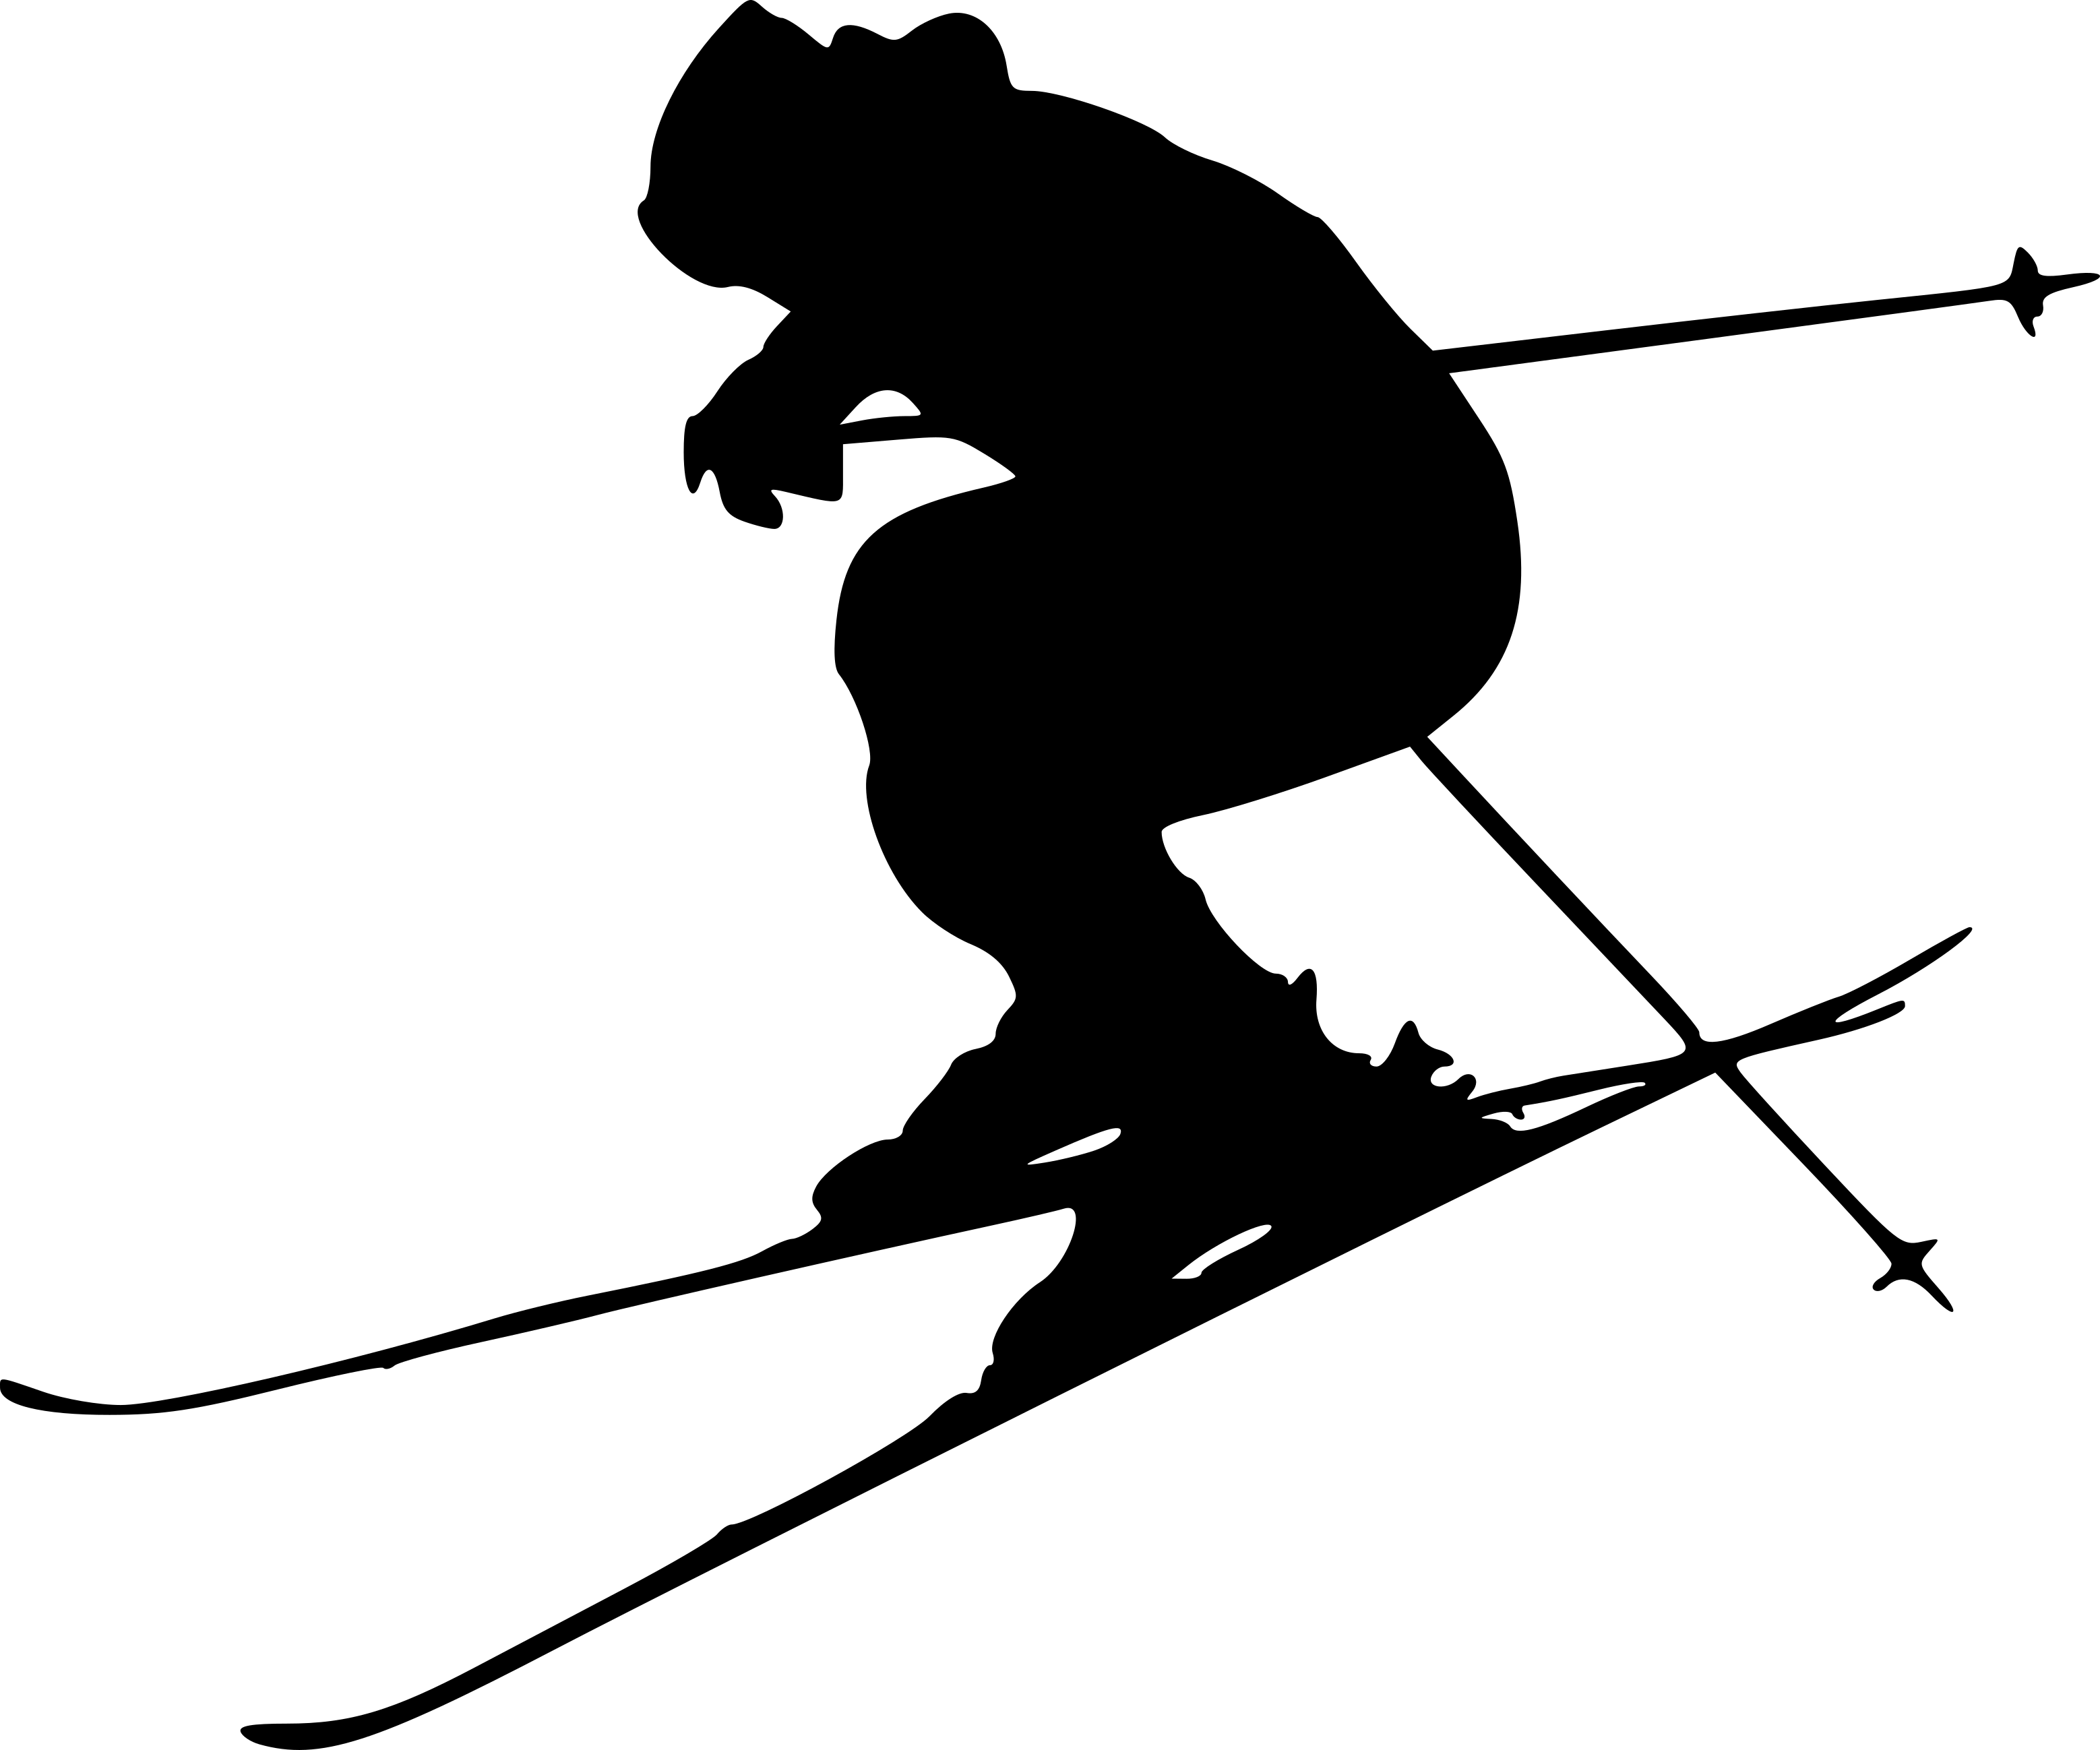
\includegraphics[scale = 0.1]{SGD.png}
\end{transitionframe}


\begin{frame}{Как обучать нейросеть?}
\begin{wideitemize}
	\item  Нейросеть - сложная функция, зависящая от весов $W$ 
	\item «Тренировка» — поиск оптимальных $W$ 
	\item «Оптимальных» — минимизирующих какой-то функционал 
	\item Какими бывают функционалы: MSE, MAE, logloss и многие другие 
	\item Как оптимизировать: \alert{градиентный спуск} 
\end{wideitemize} 
\end{frame}


\begin{frame}{Градиентный спуск}
\begin{center}
	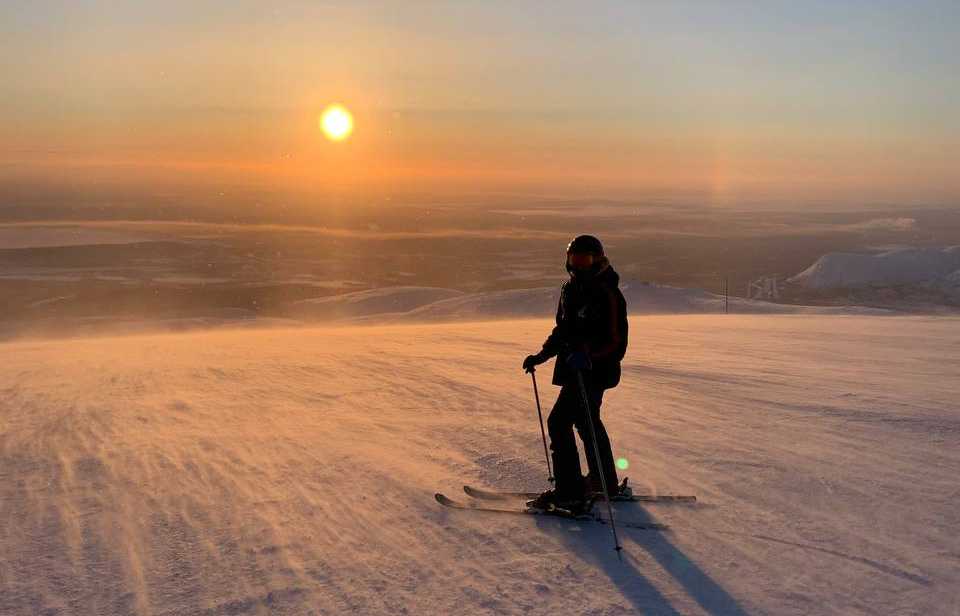
\includegraphics[width=.75\linewidth]{hb.jpg}
\end{center}
\end{frame}


\begin{frame}[fragile]{Градиентный спуск (GD)}
Проблема оптимизации: 

\[   
L(w) = \frac{1}{n} \cdot \sum_{i=1}^n L(w, x_i, y_i) \to \min_{w}
\]

\pause
Градиент указывает направление максимального роста

\[   
\nabla L(w) = \left( \frac{\partial L(w)}{\partial w_0},  \frac{\partial L(w)}{\partial w_2}, \ldots, \frac{\partial L(w)}{\partial w_k} \right)
\]

\pause 
Идём в противоположную сторону: 

\[
w_t =  \underset{{\color{red} \text{скорость обучения}}}{ w_{t-1} -   {\color{red} \eta }\cdot \nabla L(w_{t-1})} 
\]
\end{frame}


\begin{frame}[fragile]{Градиентный спуск (GD)}
Проблема оптимизации: 

\[   
L(w) = \sum_{i=1}^n L(w, x_i, y_i) \to \min_{w}
\]

Инициализация $w_0$ 
\mint{python}{while True:}
\hspace{15pt} $g_t = \frac{1}{n}\sum_{i=1}^n  \nabla L(w, x_i, y_i)$ \\
\pgr{\hspace{15pt}} $w_t = w _{t-1} - \eta_t \cdot g_t $ \\
\pgr{\hspace{15pt} if} $||w_t - w_{t-1}|| < \varepsilon:$ \\
\pgr{\hspace{30pt} break}
\end{frame}


\begin{frame}[fragile]{Сходимость}

\begin{wideitemize}
\item Останавливаем процесс, если  $$ || w_t - w_{t-1}|| < \varepsilon $$

\item  Другой вариант: $$ || \nabla L(w_t) || < \varepsilon $$

\item Обычно в глубоком обучении: останавливаемся, когда ошибка на валидационной выборке перестаёт убывать 
\end{wideitemize}
\end{frame}


\begin{frame}{Градиентный спуск}
\begin{center}
	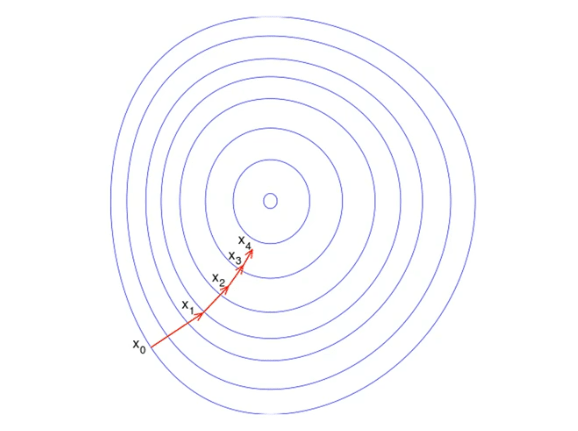
\includegraphics[width=.6\linewidth]{2dgrad.png}
\end{center}

%	\centering
%	\begin{tikzpicture}[samples=100,smooth]
%	\begin{scope}
%	\clip(-4,-1) rectangle (4,4);
%	\draw plot[domain=0:360] ({cos(\x)*sqrt(20/(sin(2*\x)+2))},{sin(\x)*sqrt(20/(sin(2*\x)+2))});
%	\draw plot[domain=0:360] ({cos(\x)*sqrt(16/(sin(2*\x)+2))},{sin(\x)*sqrt(16/(sin(2*\x)+2))});
%	\draw plot[domain=0:360] ({cos(\x)*sqrt(12/(sin(2*\x)+2))},{sin(\x)*sqrt(12/(sin(2*\x)+2))});
%	\draw plot[domain=0:360] ({cos(\x)*sqrt(8/(sin(2*\x)+2))},{sin(\x)*sqrt(8/(sin(2*\x)+2))});
%	\draw plot[domain=0:360] ({cos(\x)*sqrt(4/(sin(2*\x)+2))},{sin(\x)*sqrt(4/(sin(2*\x)+2))});
%	\draw plot[domain=0:360] ({cos(\x)*sqrt(1/(sin(2*\x)+2))},{sin(\x)*sqrt(1/(sin(2*\x)+2))});
%	\draw plot[domain=0:360] ({cos(\x)*sqrt(0.0625/(sin(2*\x)+2))},{sin(\x)*sqrt(0.0625/(sin(2*\x)+2))});
%	
%	\draw[-latex new,arrow head=0.25cm,blue,ultra thick] (-2,3.65) to (-1.93,3);
%	\draw[-latex new,arrow head=0.25cm,blue,ultra thick] (-1.93,3) to (-1.75,2.4);
%	\draw[-latex new,arrow head=0.25cm,blue,ultra thick] (-1.75,2.4) to (-1.5,1.8);
%	\draw[-latex new,arrow head=0.25cm,blue,ultra thick] (-1.5,1.8) to (-1.15,1.3);
%	
%	\node at (-1.4,3.8){$w[0]$};
%	\node at (-1.2,3.2){$w[1]$};
%	\node at (-1.05,2.6){$w[2]$};
%	\node at (-0.8,2){$w[3]$};
%	\node at (-0.6,1.4){$w[4]$};
%	\end{scope}
%	\end{tikzpicture}
\end{frame}


\begin{frame}[fragile]{Пример (линейная регрессия):}
Проблема оптимизации: 
\[   
L(w) = \frac{1}{n} \cdot \sum_{i=1}^n  (y_i - x_i^T w)^2 \to \min_{w}
\]

Градиент: 

\[   
\nabla L(w) =   { \only<2>{ \color{red}} -2 \cdot   \frac{1}{n} \cdot \sum_{i=1}^n (y_i - x_i^T w)\cdot x_i }
\]

Идём в противоположную сторону: 

\[
w_t =   w_{t-1}  +  0.001 \cdot  { \only<2>{ \color{red}}  2 \cdot \frac{1}{n} \cdot \sum_{i=1}^n (y_i - x_i^T w_{t-1})\cdot x_i } 
\]

\only<2>{ { \color{red} Дорого постоянно считать такие суммы по всей выборке}}
\end{frame}



\begin{frame}[fragile]{Стохастический градиентный спуск (SGD)}
Проблема оптимизации: 

\[   
L(w) = \sum_{i=1}^n L(w, x_i, y_i) \to \min_{w}
\]

Инициализация $w_0$ 
\mint{python}{while True:}
\hspace{15pt} рандомно выбрали $i$ \\
\pgr{\hspace{15pt}} $g_t = \nabla L(w_{t-1}, x_i, y_i)$ \\
\pgr{\hspace{15pt}} $w_t = w _{t-1} - \eta_t \cdot g_t  $ \\
\pgr{\hspace{15pt} if} $||w_t - w_{t-1}|| < \varepsilon:$ \\
\pgr{\hspace{30pt} break}
\end{frame}


\begin{frame}[fragile]{Пример (линейная регрессия):}
Проблема оптимизации: 
\[   
L(w) = \frac{1}{n} \cdot \sum_{i=1}^n  (y_i - x_i^T w)^2 \to \min_{w}
\]

Градиент: 

\[   
\nabla L(w) =  { \color{red} - 2 \cdot (y_i - x_i^T w)\cdot x_i }
\]

Идём в противоположную сторону: 

\[
w_{t}=   w_{t-1}  +  0.001 \cdot   {\color{red}  2 \cdot (y_i - x_i^T w_{t-1})\cdot x_i }
\]
\end{frame}


\begin{frame}{Скорость обучения в SGD} 
\begin{center}
	\resizebox{0.55\linewidth}{!}{
		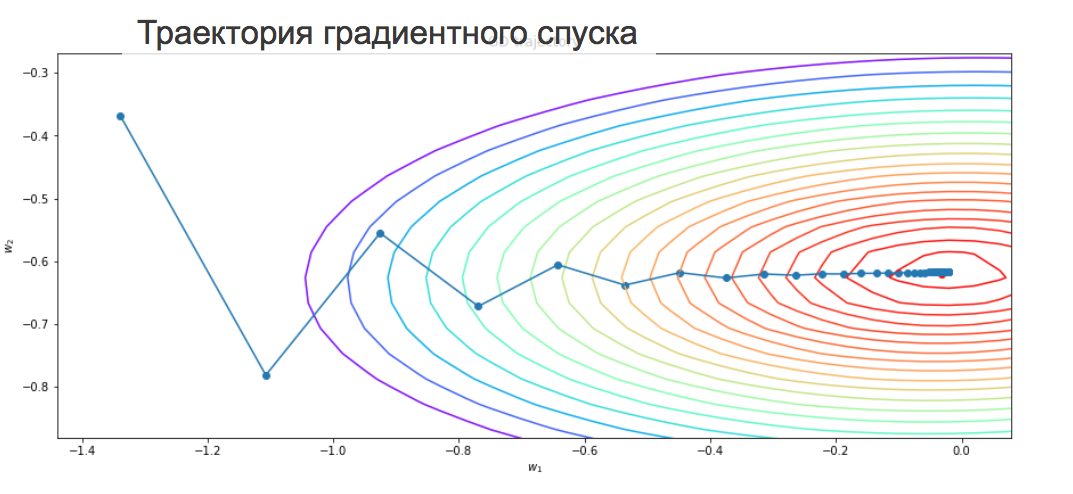
\includegraphics{gd_t.png}
	}
	
	\resizebox{0.55\linewidth}{!}{
		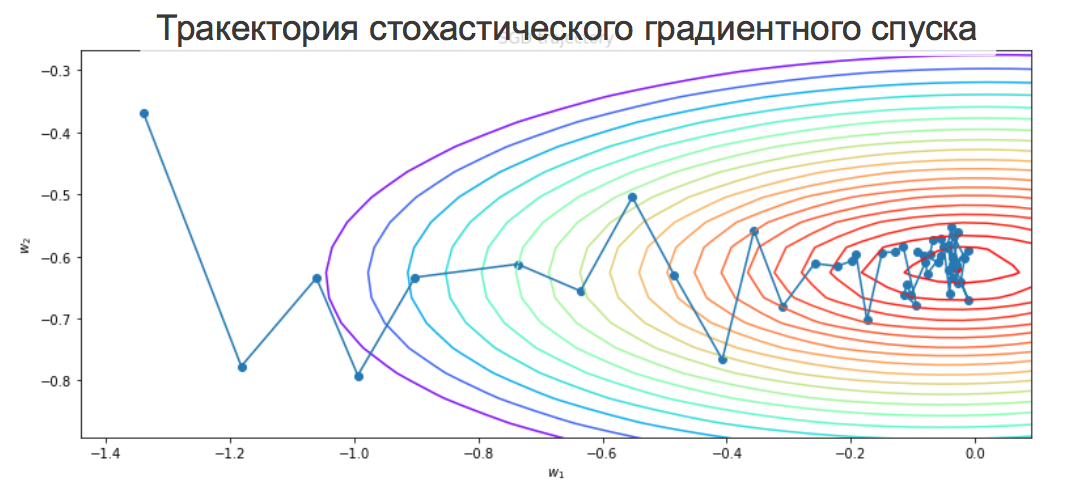
\includegraphics{sgd_t.png}
	}
\end{center}
\end{frame}


\begin{frame}{Стохастический градиентный спуск (SGD)}
\begin{wideitemize}
	\item   Можно доказать, что оценка по одному объекту несмещённая, то есть в среднем мы идём в правильную сторону
	
	\item   Даже в точке оптимума оценка по одному объекту вряд ли будет нулевой, поэтому важно, чтобы длина шага стремилась к нулю
	
	\item Длина шага  должна зависит от номера итерации следующим образом:
	
	\[
	\sum_{t=0}^{\infty} \eta_t = \infty \qquad  \sum_{t=0}^{\infty} \eta_t^2 < \infty
	\]
	
	\item   Сходимость к глобальному минимуму гарантируется только для выпуклых функций
\end{wideitemize}
\end{frame}


\begin{frame}{Скорость обучения в SGD} 

\[ 
\eta_t = \frac{0.1}{t^{0.3}}
\]

\begin{center}
	\resizebox{0.8\linewidth}{!}{
		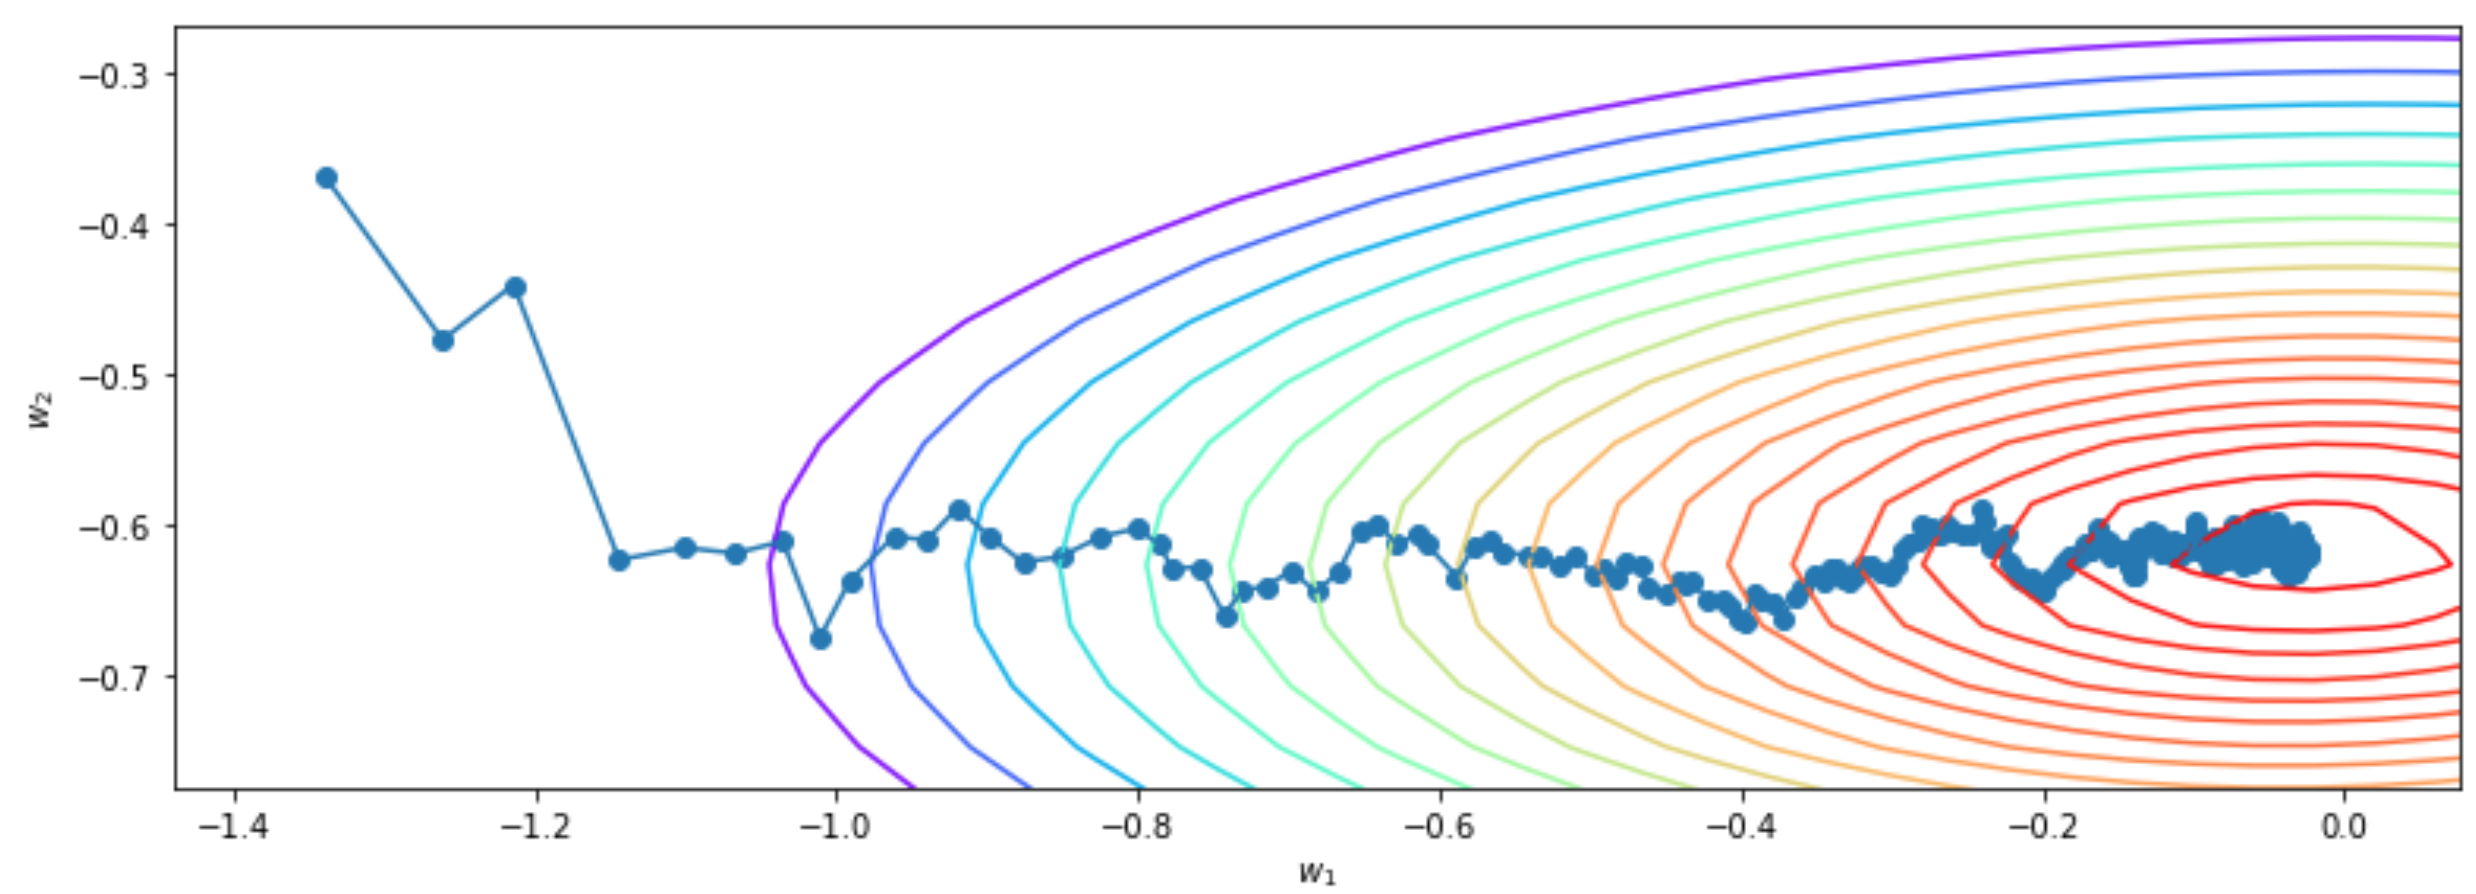
\includegraphics{sgd_t2.png}
	}

\alert{Мы инженеры и используем то, что работает}
\end{center}
\end{frame}



\begin{frame}{GD vs SGD}
\begin{columns}[T] %
	\begin{column}{.5\textwidth}
		\resizebox{0.95\linewidth}{!}{
			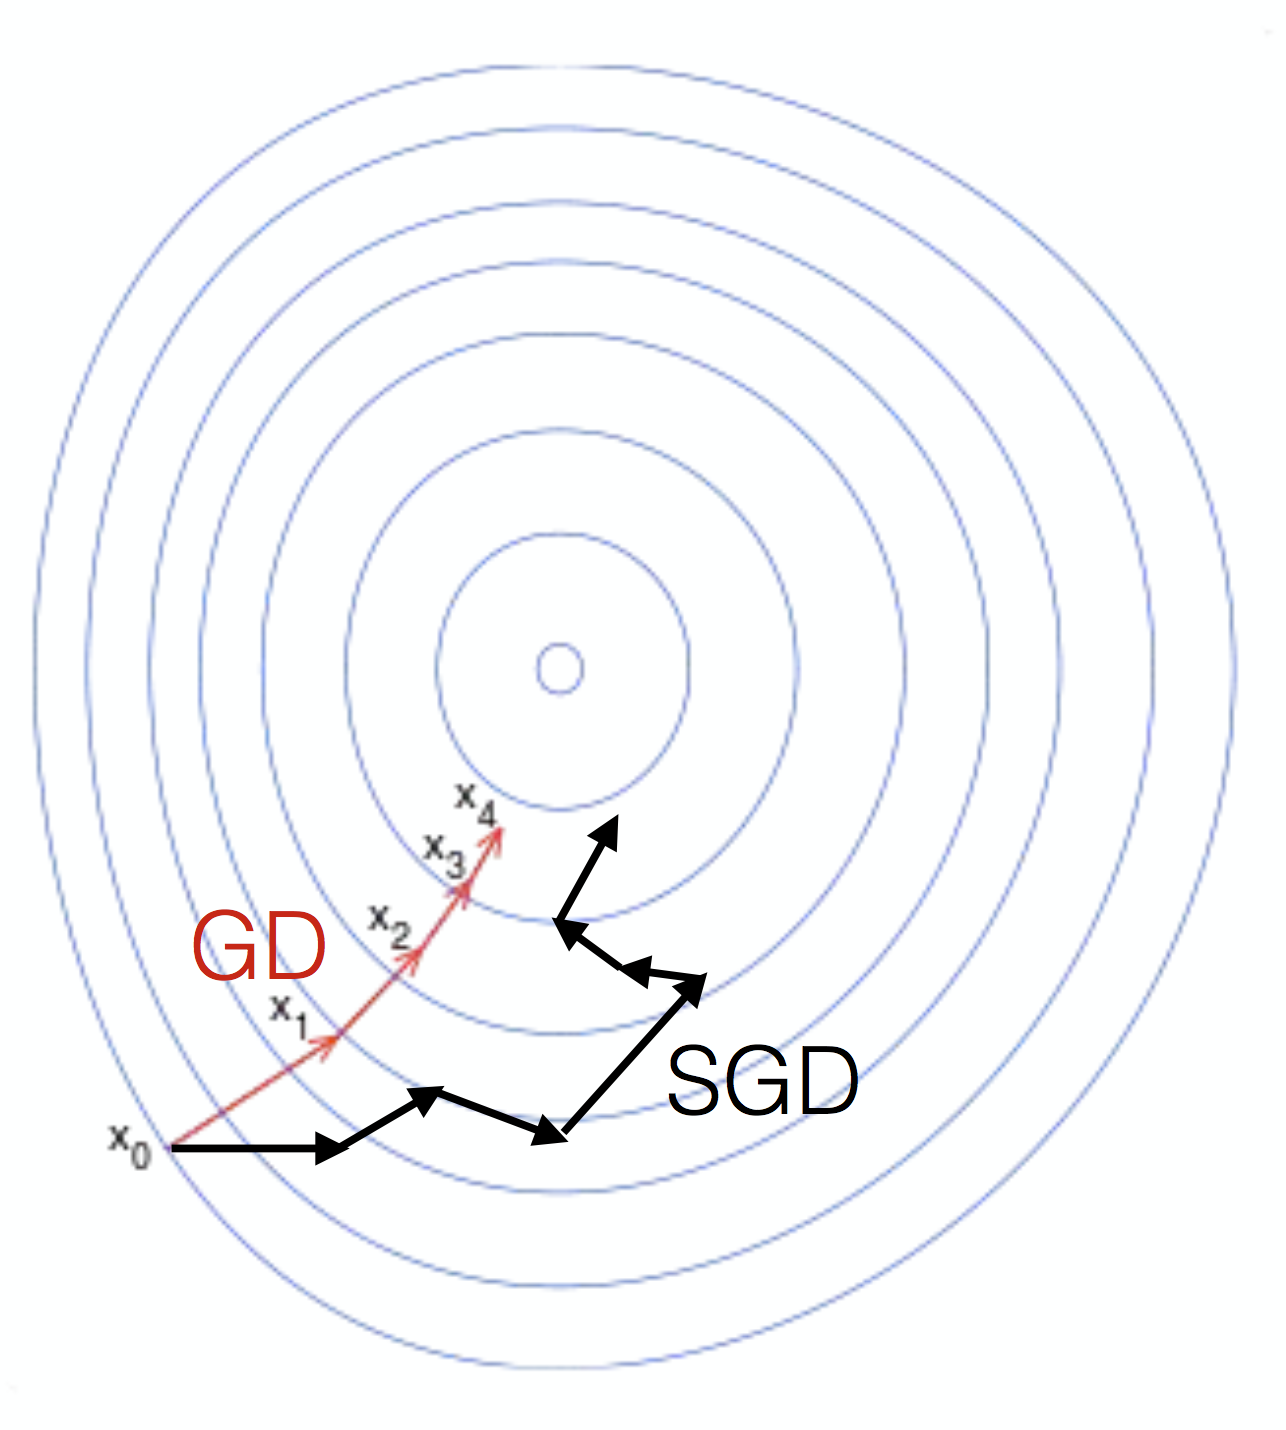
\includegraphics{st2grad.png}
		}
	\end{column}%
	\hfill%
	\begin{column}{.5\textwidth}
		\begin{wideitemize}
			\item И для GD и для SGD нет гарантий глобального минимума, сходимости
			\item SGD быстрее,на каждой итерации используется только одно наблюдение
			\item Для SGD спуск очень зашумлён 
			\item  GD: $O(n)$, SGD: $O(1)$
			\item Шум в оценке градиента помогает выпрыгивать из локальных оптимумов
		\end{wideitemize}
	\end{column}%
\end{columns}
\end{frame}


\begin{frame}[fragile]{Mini-bath SGD}
	Проблема оптимизации: 
	
	\[   
	L(w) = \sum_{i=1}^n L(w, x_i, y_i) \to \min_{w}
	\]
	
	Инициализация $w_0$ 
	\mint{python}{while True:}
	\pgr{\hspace{15pt}} рандомно выбрали $m < n$ объектов \\
	\pgr{\hspace{15pt}} $g_t =\frac{1}{m}\sum_{i=1}^m  \nabla L(w, x_i, y_i)$ \\
	\pgr{\hspace{15pt}} $w_t = w _{t-1} - \eta_t \cdot g_t   $ \\
	\pgr{\hspace{15pt} if} $||w_t - w_{t-1}|| < \varepsilon:$ \\
	\pgr{\hspace{30pt} break}
\end{frame}


\begin{frame}{Mini-bath SGD}
	\begin{wideitemize}
		\item Размер батча обычно десятки или сотни наблюдений
	
		\item Имеет смысл брать степень двойки
		
		\item Возможно, делает оценку градиента более стабильной 
		
		\item За счёт векторизации также эффективен, как шаг по одному объекту 
	\end{wideitemize}
\end{frame}



\begin{frame}{Mini-bath SGD (2018)}
\begin{center}
	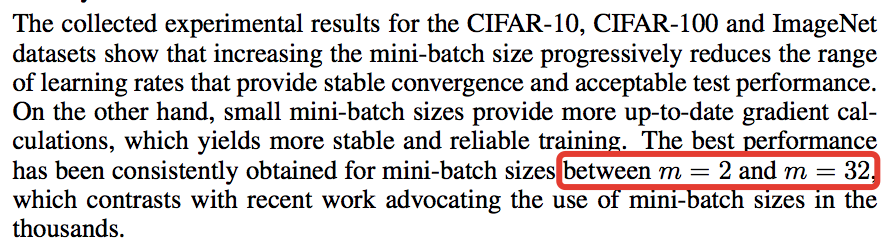
\includegraphics[width=0.95\paperwidth]{mini_batch.png}
\end{center}
\vfill %
\footnotesize 
\color{blue} \url{https://arxiv.org/abs/1804.07612}
\end{frame}


\begin{frame}{Mini-bath SGD (2018)}
\begin{center}
	
\includegraphics[width=0.8\paperwidth]{lec_meme.png}
\end{center}
\vfill %
\footnotesize 
\color{blue} \url{https://arxiv.org/abs/1804.07612}
\end{frame}


%\begin{frame}{Large batch optimization (2020) }
%%\begin{center}
%%	
\includegraphics[width=0.8\paperwidth]{lec_meme.png}
%%\end{center}
%\vfill %
%\footnotesize 
%\color{blue} \url{https://arxiv.org/abs/1904.00962}
%\end{frame}


\begin{frame}{Скорость обучения}
\begin{wideitemize}
	\item Скорость обучения $\eta$ надо подбирать аккуратно, если она будет большой, мы можем скакать вокруг минимума, если маленькой - вечно ползти к нему
	
	\begin{center}
		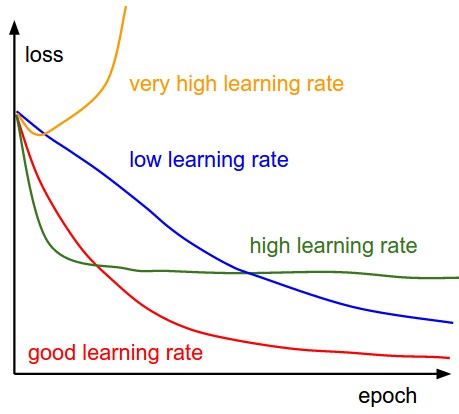
\includegraphics[width=0.37\paperwidth]{learningrates.jpg}
	\end{center}
\end{wideitemize}
\end{frame}


\begin{frame}{Боб чилит в локальном минимуме}
\begin{center}
	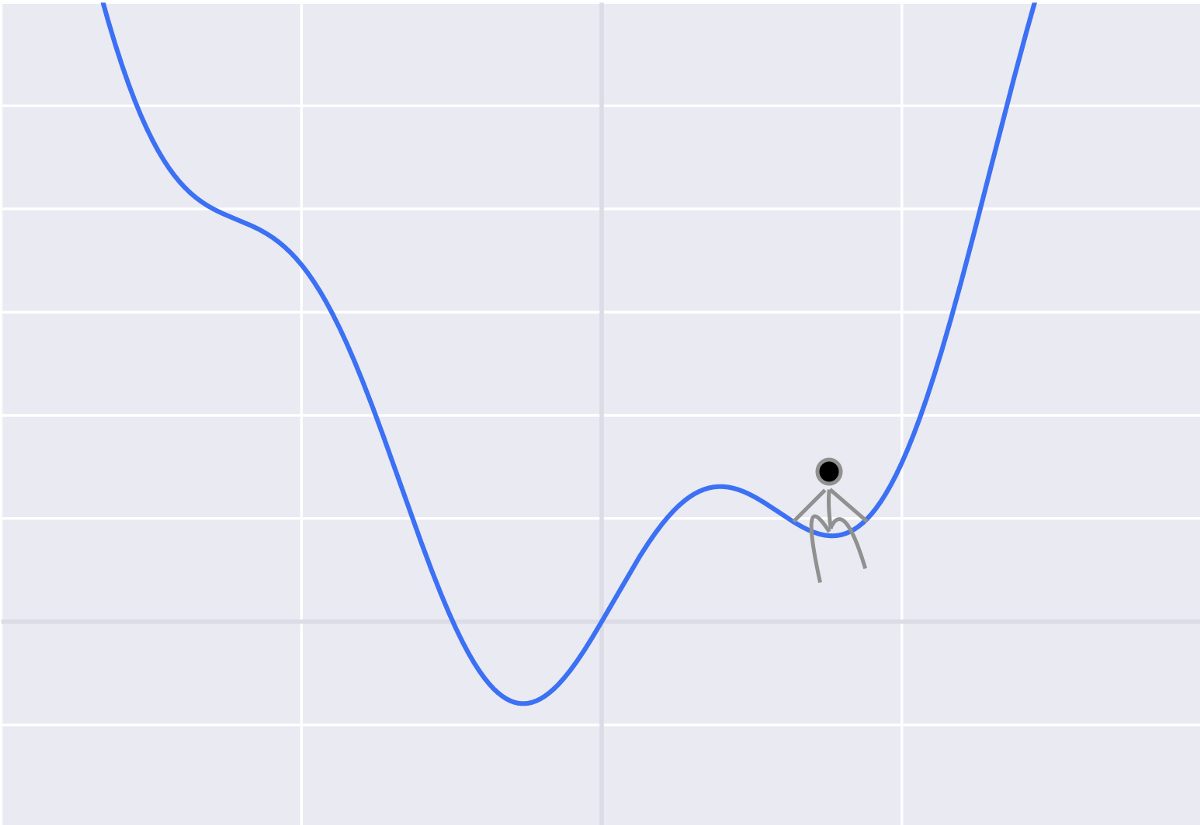
\includegraphics[width=0.6\paperwidth]{bob_local_chill.png}
\end{center}
\vfill %
\footnotesize 
\color{blue} \url{https://hackernoon.com/life-is-gradient-descent-880c60ac1be8}
\end{frame}


\begin{frame}{Седловые точки}
\begin{center}
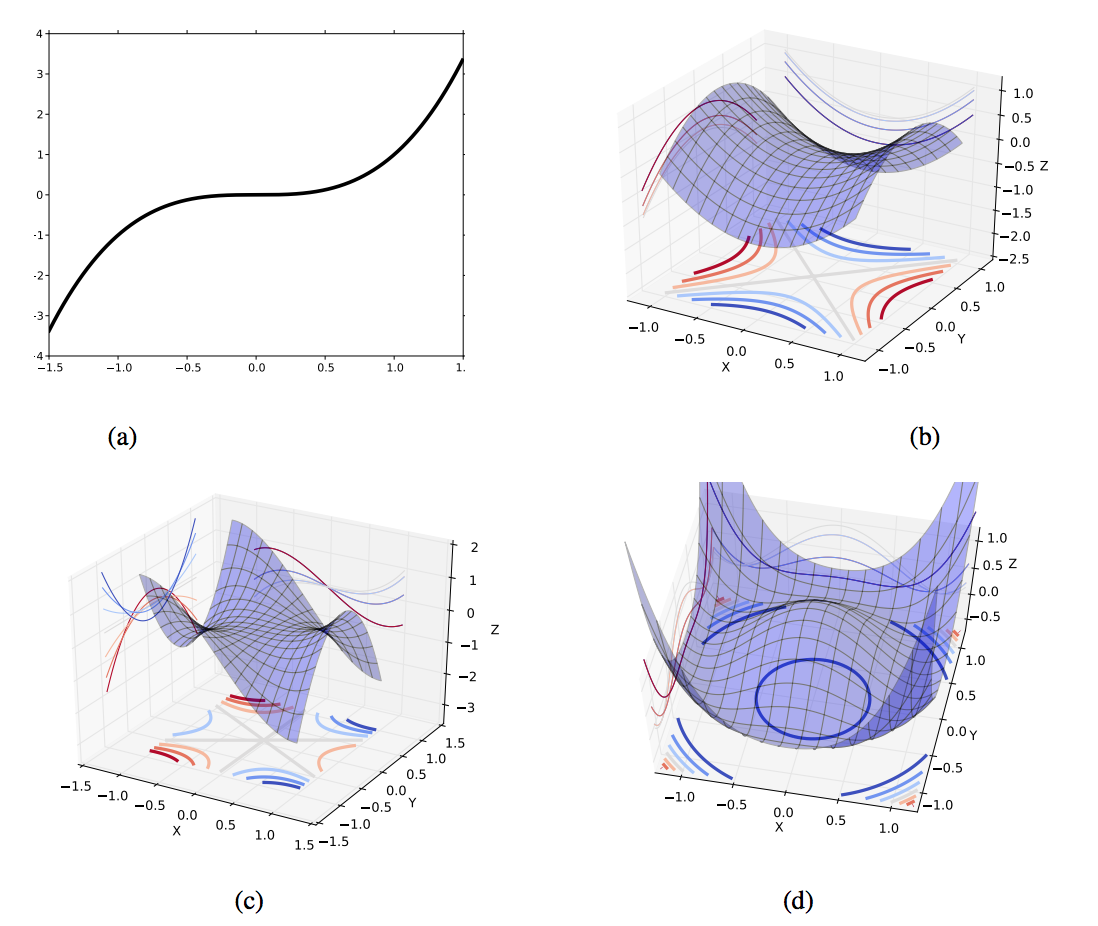
\includegraphics[width=0.5\paperwidth]{sedlo.png}
\end{center}
\vfill %
\footnotesize 
\color{blue} \url{https://arxiv.org/pdf/1406.2572.pdf}
\end{frame}


\begin{frame}{Визуализация потерь}
\begin{center}
	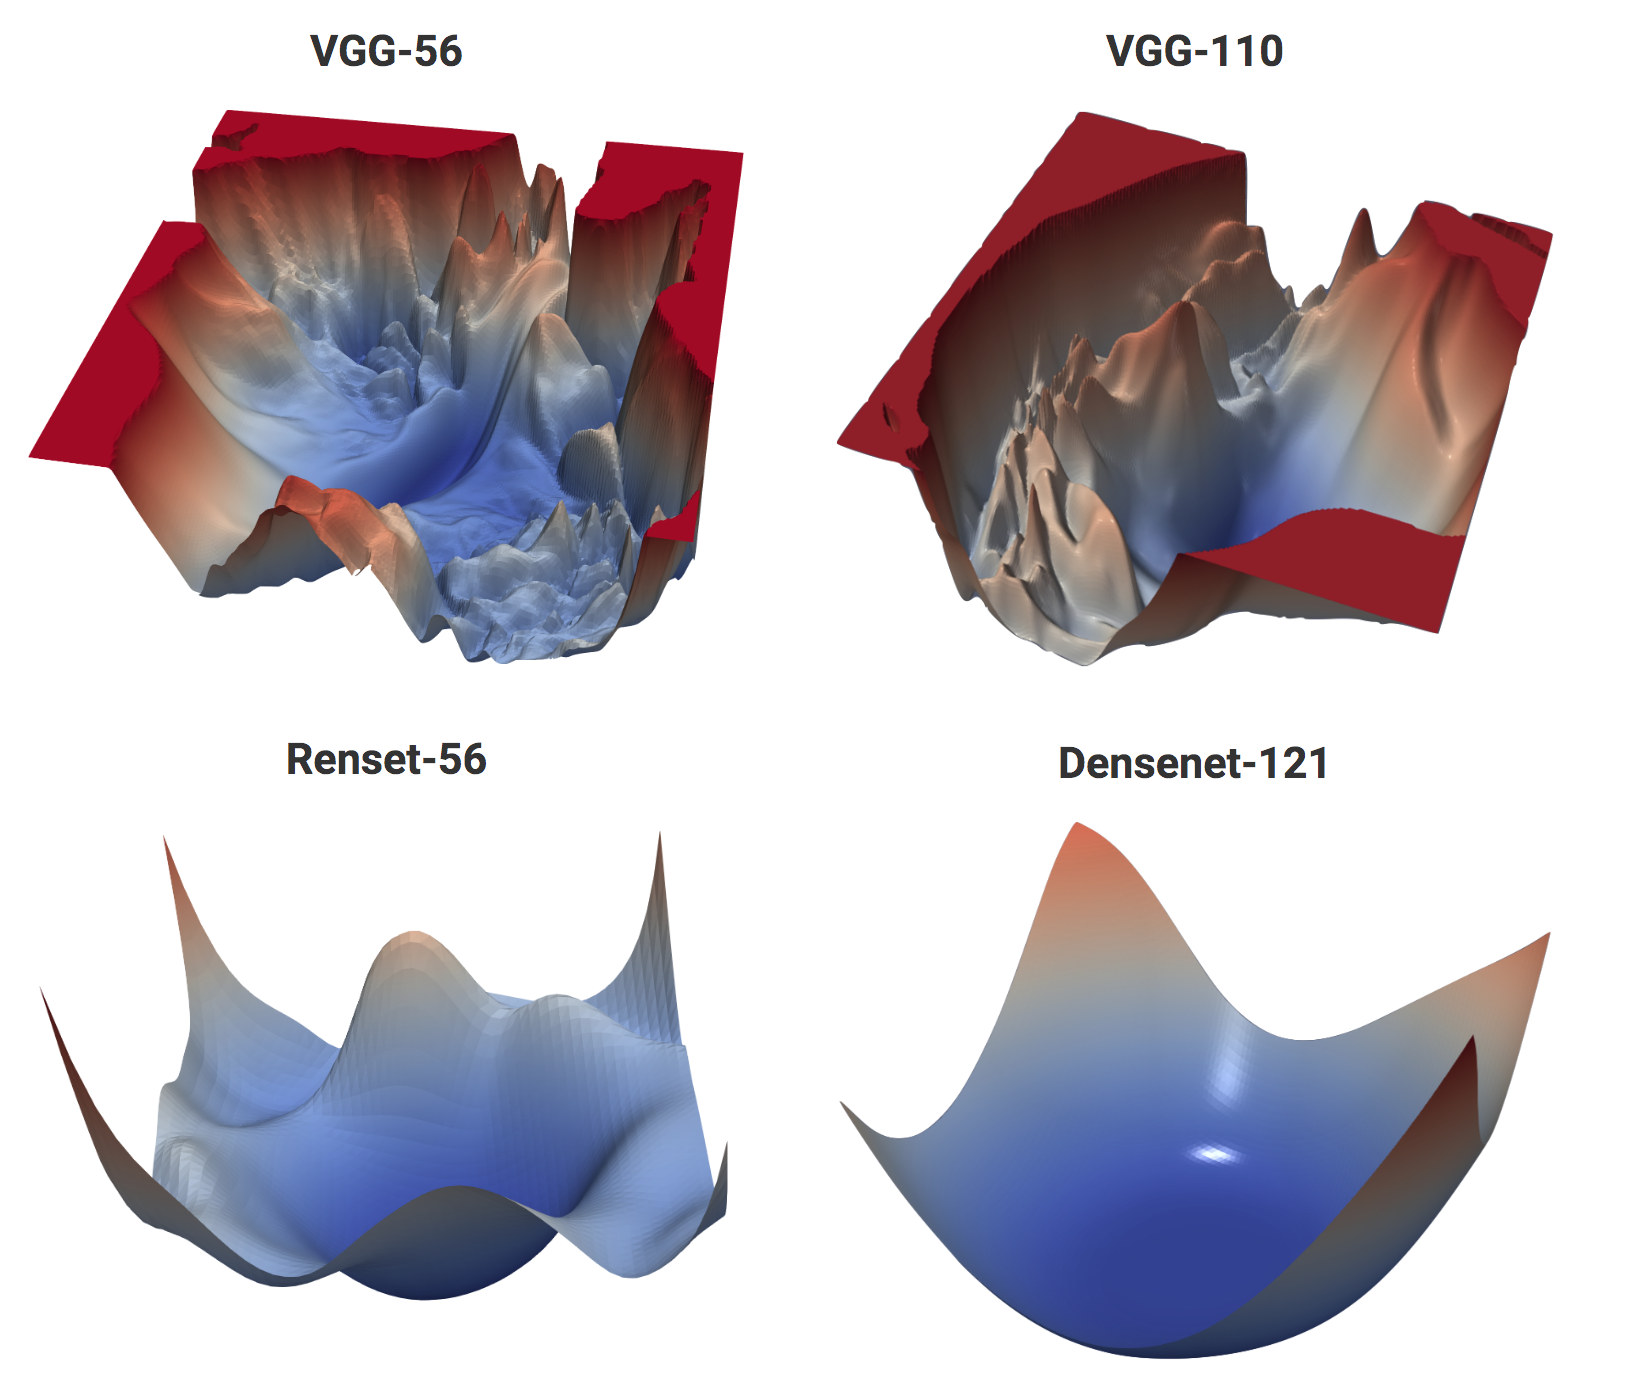
\includegraphics[width=0.5\paperwidth]{loss.png}
\end{center}
\vfill %
\footnotesize 
\color{blue} \url{https://arxiv.org/pdf/1712.09913.pdf} \newline  \url{https://github.com/tomgoldstein/loss-landscape}
\end{frame}


\begin{transitionframe}
	\begin{center}
		\Huge 50 оттенков градиентного спуска
	\end{center}
	\centering 
\includegraphics[scale = 0.1]{shadows50.jpg}
\end{transitionframe}


\begin{frame}[fragile]{Mini-bath SGD}
Проблема оптимизации: 

\[   
L(w) = \sum_{i=1}^n L(w, x_i, y_i) \to \min_{w}
\]

Инициализация $w_0$ 
\mint{python}{while True:}
\pgr{\hspace{15pt}} рандомно выбрали $m < n$ индексов \\
\pgr{\hspace{15pt}} $g_t =\frac{1}{m}\sum_{i=1}^m  \nabla L(w, x_i, y_i)$ \\
\pgr{\hspace{15pt}} $w_t = w _{t-1} - \eta_t \cdot g_t   $ \\
\pgr{\hspace{15pt} if} $||w_t - w_{t-1}|| < \varepsilon:$ \\
\pgr{\hspace{30pt} break}
\end{frame}


\begin{frame}[fragile]{Вызовы}
\begin{wideitemize}
\item Скорость обучения $\eta$ надо подбирать аккуратно, если она будет большой, мы можем скакать вокруг минимума, если маленькой - вечно ползти к нему.

\begin{center}
	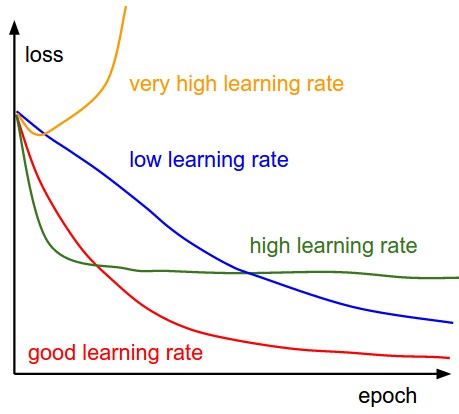
\includegraphics[width=0.25\paperwidth]{learningrates.jpg}
\end{center}

\item К обновлению всех параметров применяется одна и та же скорость обучения. Возможно, что какие-то параметры приходят в оптимальную точку быстрее, и их не надо обновлять.
\end{wideitemize}
\end{frame}


\begin{frame}{Momentum SGD}
Мы считали на каждом шаге градиент по формуле  \[g_t =\frac{1}{m}\sum_{i=1}^m  \nabla L(w_{t-1}, x_i, y_i)\] После шага мы забывали его, {\color{red} давайте запоминать направление:} 

\begin{equation*}
\begin{aligned}
h_t &= \alpha \cdot h_{t-1} + \eta \cdot g_t \\
w_t &= w_{t-1} - h_t
\end{aligned}	
\end{equation*}

\begin{itemize}
\item Движение поддерживается в том же направлении
\item Нет резких изменений направления движения
\item Обычно $\alpha = 0.9$.
\end{itemize}
\vfill
\footnotesize
Крутой интерактив для моментума: {\color{blue} \url{https://distill.pub/2017/momentum/}}
\end{frame}


\begin{frame}{Momentum SGD}
\begin{wideitemize}
\item Бежим с горки и всё больше ускоряемся в том направлении, в котором были направлены сразу несколько предыдущих градиентов, но при этом движемся медленно там, где градиент постоянно меняется
\item Хотелось бы не просто бежать с горы, но и хотя бы на полшага смотреть себе под ноги, чтобы внезапно не споткнуться $\Rightarrow$  \alert{давайте смотреть на градиент в будущей точке}
\item Согласно методу моментов $\alpha \cdot h_{t-1}$ точно будет использоваться при шаге, давайте искать $\nabla L(w_{t-1} - \alpha \cdot h_{t-1})$.
\end{wideitemize}
\end{frame}


\begin{frame}{Nesterov Momentum SGD}
\begin{itemize}
\item Мы теперь сначала прыгаем в том же направлении, в каком шли до этого, потом корректируем его (голубая траектория).
\end{itemize}
\begin{center}
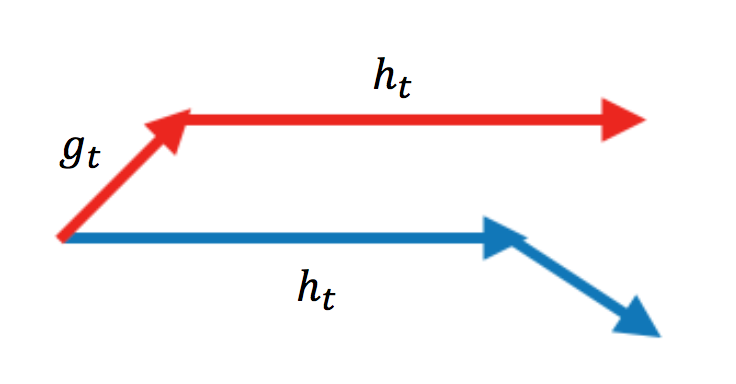
\includegraphics[width=.4\linewidth]{nesterov.png}
\end{center}
\begin{equation*}
\begin{aligned}
h_t &= \alpha \cdot h_{t-1} + \eta \cdot \nabla L(w_{t-1} - \alpha \cdot h_{t-1}) \\
w_t &= w_{t-1} - h_t
\end{aligned}	
\end{equation*}
\end{frame}


\begin{frame}{Разная скорость обучения}
\begin{wideitemize}
\item Может сложиться, что некоторые веса уже близки к своим локальным минимумам, по этим координатам надо двигаться медленнее, а по другим быстрее $\Rightarrow$ {\color{red} адаптивные методы градиентного спуска }

\item Шаг изменения должен быть меньше у тех параметров, которые в большей степени варьируются в данных, и больше у тех, которые менее изменчивы 
\end{wideitemize}
\end{frame}


\begin{frame}{AdaGrad}
\begin{equation*}
\begin{aligned}
G_t^j &= G_{t-1}^j + g_{tj}^2 \\
w_t^j &= w_{t-1}^j - \frac{\eta}{\sqrt{G_t^j + \varepsilon}} \cdot g_t^j
\end{aligned}	
\end{equation*}
\begin{wideitemize}
\item  $g_t^j$ — градиент по $j-$ому параметру
\item своя скорость обучения для каждого параметра
\item обычно $\eta = 0.01$, т.к. параметр не очень важен
\item $G_t^j$ всегда увеличивается, из-за этого обучение может рано останавливаться $\Rightarrow$  RMSprop
\end{wideitemize}
\end{frame}


\begin{frame}{RMSprop}
\begin{equation*}
\begin{aligned}
G_t^j &= \alpha \cdot G_{t-1}^j + (1 - \alpha) \cdot g_{tj}^2 \\
w_t^j &= w_{t-1}^j - \frac{\eta_t}{\sqrt{G_t^j + \varepsilon}} \cdot g_t^j
\end{aligned}	
\end{equation*}
\begin{wideitemize}
\item Обычно $ \alpha = 0.9$
\item Скорость обучения адаптируется к последнему сделанному шагу, бесконтрольного роста $G_t^j$ больше не происходит 
\item RMSprop нигде не был опубликован, Хинтон просто привёл его в своей лекции, сказав, что это норм тема
\end{wideitemize}
\end{frame}


\begin{frame}{Adam (Adaptive Moment Estimation)}
\begin{wideitemize} 
	\item Комбинируем Momentum и индивидуальные скорости обучения
\end{wideitemize}
\begin{equation*}
\begin{aligned}
h_t^j &= \frac{\beta_1 \cdot h_{t-1}^j + (1 - \beta_1) \cdot g_{tj}}{1 - \beta_1^t} \\
G_t^j &= \frac{\beta_2 \cdot G_{t-1}^j + (1 - \beta_2) \cdot g_{tj}^2}{1 - \beta_2^t} \\
w_t^j &= w_{t-1}^j - \frac{\eta_t}{\sqrt{G_t^j + \varepsilon}} \cdot h_t^j
\end{aligned}	
\end{equation*}
\begin{wideitemize} 
\item Фактически $h_t$ и $G_t$ это оценки первого и второго моментов для стохастического градиента
\end{wideitemize}

\end{frame}


\begin{frame}{Сравнение на MNIST}
\begin{center}
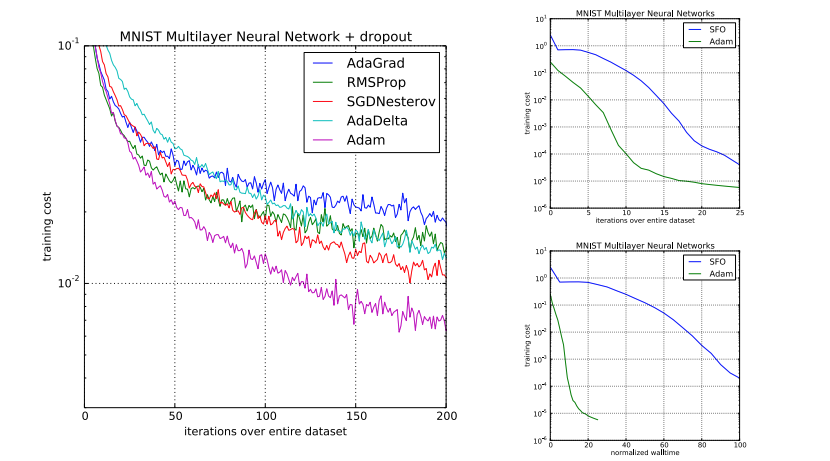
\includegraphics[scale=0.4]{adam_mnist.png}
\end{center}
\vfill %
\footnotesize
{\color{blue} \url{https://arxiv.org/pdf/1412.6980.pdf}}
\end{frame}




\begin{frame}{Резюме по методам градиентного спуска}
\begin{wideitemize}
\item Momentum SGD сохраняет направление шага и позволяет добиваться более быстрой сходимости
\item  Адаптивные методы позволяют находить индивидуальную скорость обучения для каждого параметра
\item Adam комбинирует в себе оба подхода
\item Давайте посмотрим \href{http://ruder.io/content/images/2016/09/contours_evaluation_optimizers.gif}{визуализацию 1} и \href{http://ruder.io/content/images/2016/09/saddle_point_evaluation_optimizers.gif}{визуализацию 2}
\item \alert{В будущих лекциях мы продолжим разговор про то, как можно улучшить методы оптимизации нейронных сетей.} 
\end{wideitemize}
\end{frame}



\begin{transitionframe}
	\begin{center}
		\Huge Эпохи, батчи, ранняя остановка
	\end{center}
	\centering 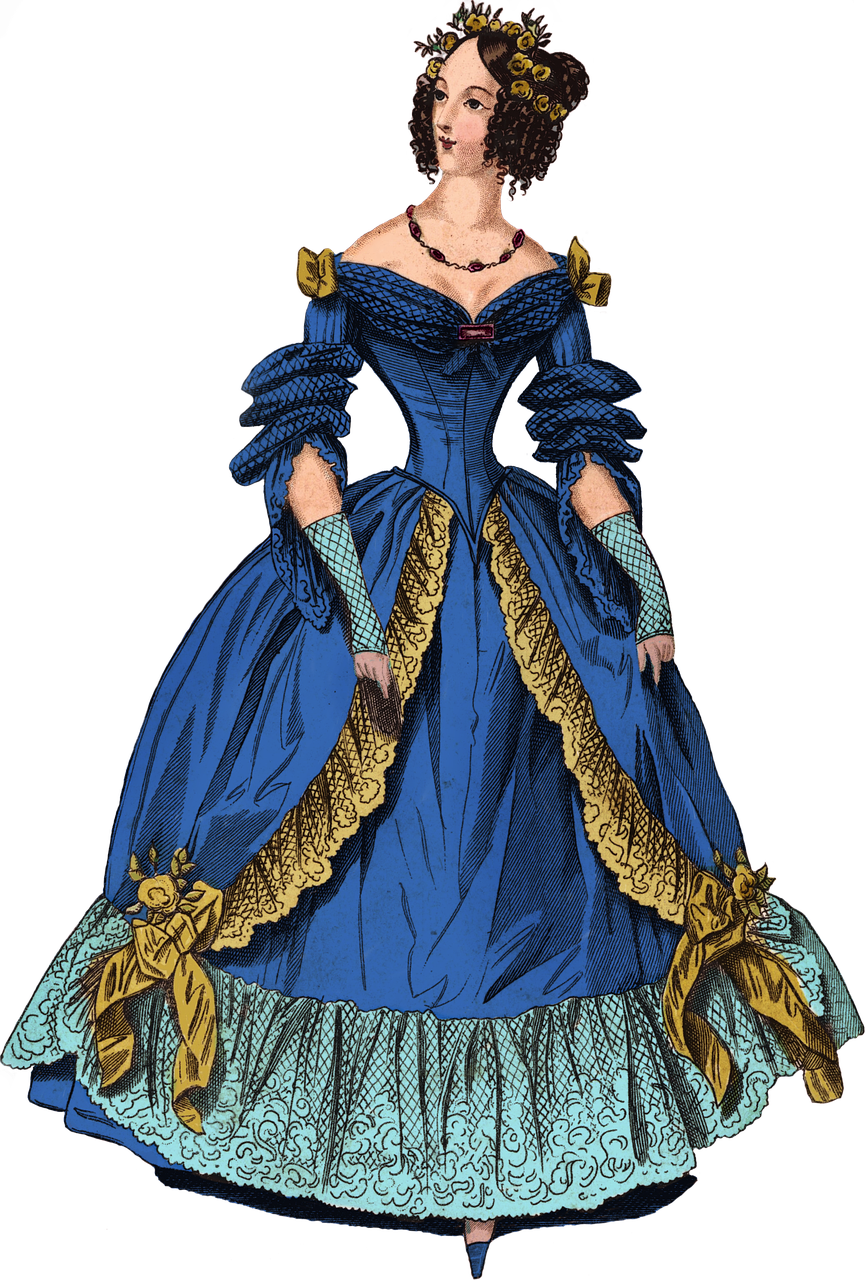
\includegraphics[scale = 0.08]{epocha.png}
\end{transitionframe}


\begin{frame}{Нейросети и кросс-валидация}
\begin{wideitemize}
	\item Кросс-валидацию для нейронных сетей обычно не делают 
	
	\item Сетка учится долго, дробить выборку на части и обучать несколько экземпляров очень дорого
	
	\item Перебор гиперпараметров по решётке обычно не делают, так как это тоже дорого
	
	\item При экспериментах делают одно какое-то изменение за раз и запускают обучение
\end{wideitemize}	
\end{frame}


\begin{frame}{Эпохи и батчи}
	\begin{center}
		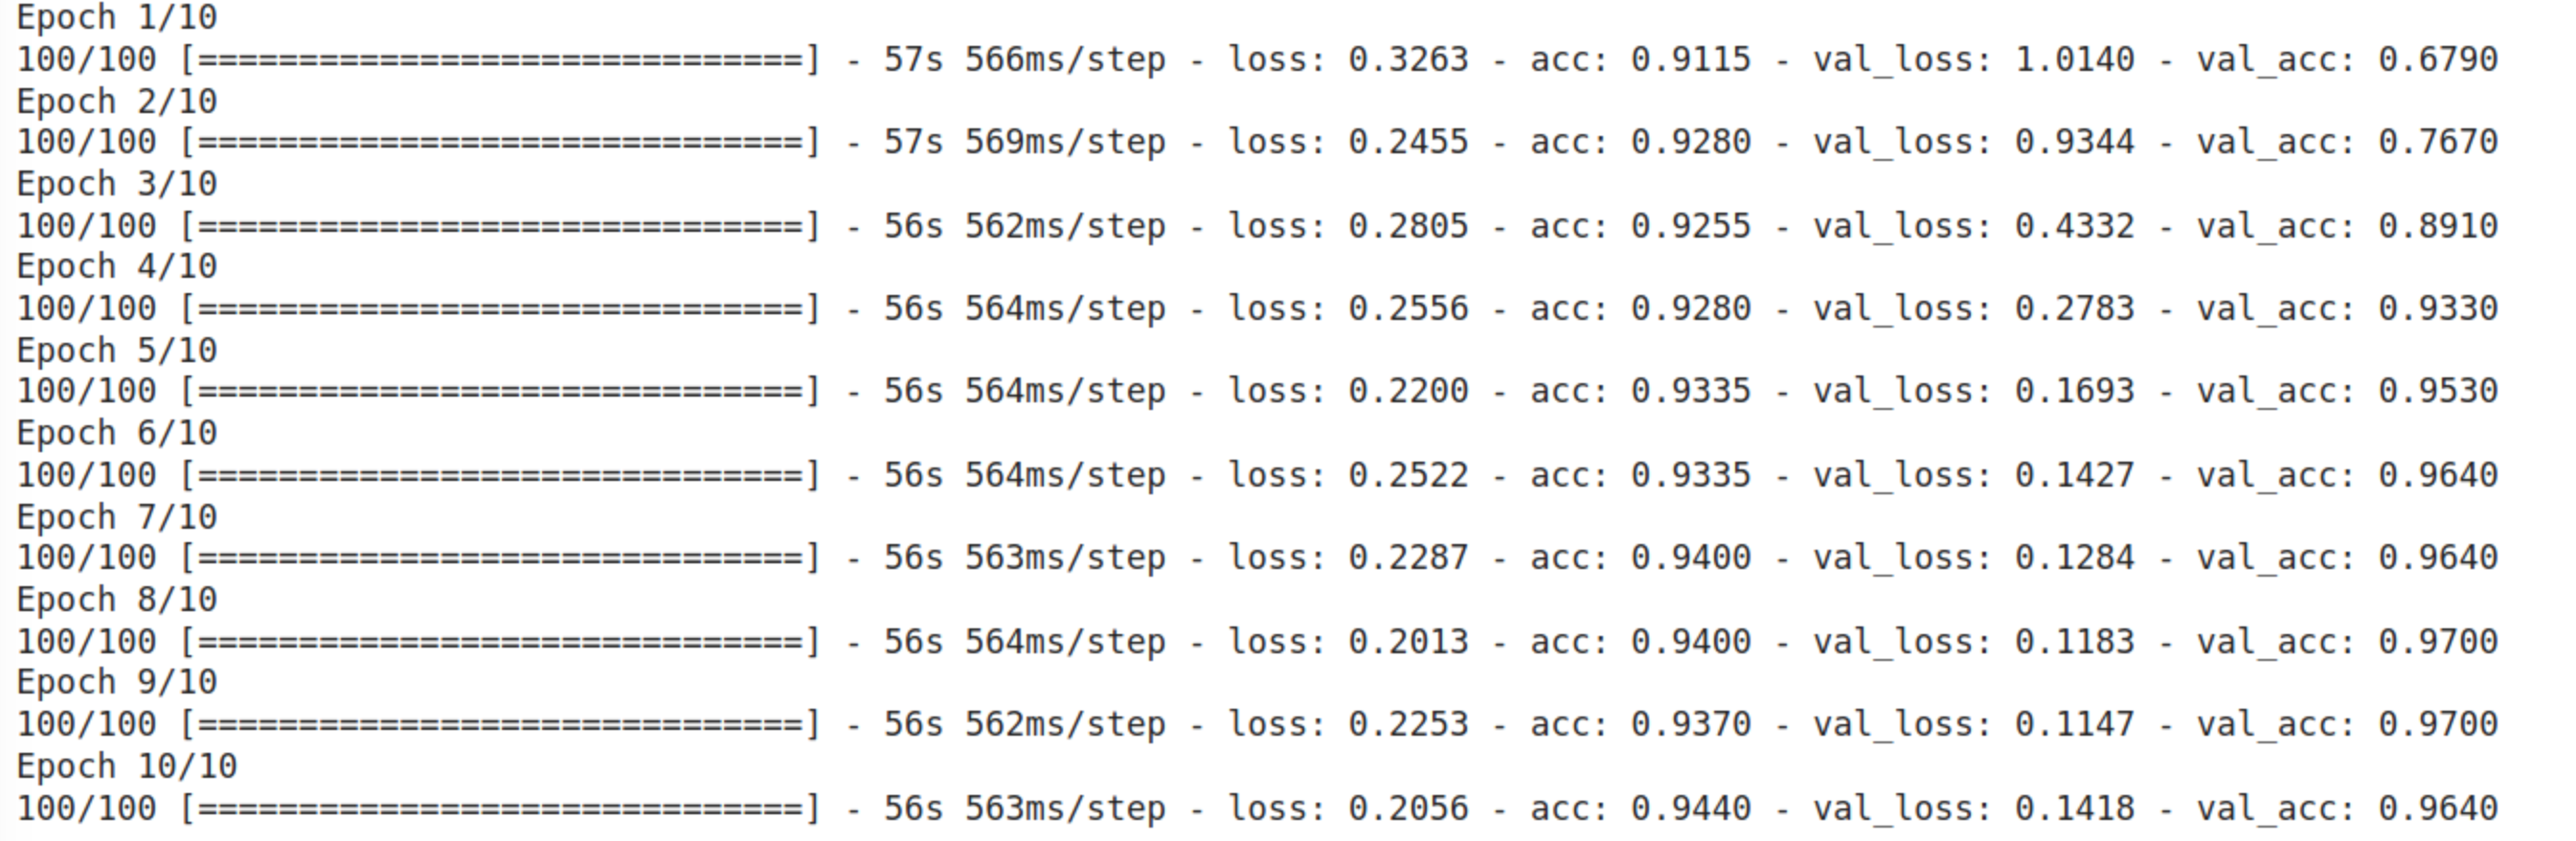
\includegraphics[width=.95\linewidth]{epoch_batch.png}
	\end{center}
	\begin{itemize}
		\item \alert{Эпоха} — один проход по данным 
		\item \alert{Батч} — маленький кусочек данных
		\item \alert{Перед каждой эпохой данные надо перемешивать}
	\end{itemize}
\end{frame}


\begin{frame}{Как отслеживать обучение? Графики!}
\begin{wideitemize}
	\item Значение функции потерь в зависимости от итерации (проверка идёт ли оптимизация)
	
	\item Обучающая выборка не покажет переобучение $\Rightarrow$ следим за ошибкой на валидационной выборке
	
	\item \alert{ВАЖНО:}  использовать валидацию, а не тест
	
	\item Число эпох для обучения - гиперпараметр, на валидации можно понять, когда надо остановить обучение
	
	\item На тестовой выборке оцениваем окончательное качество модели	
\end{wideitemize}
\end{frame}


\begin{frame}{Переобучение}
\begin{center}
	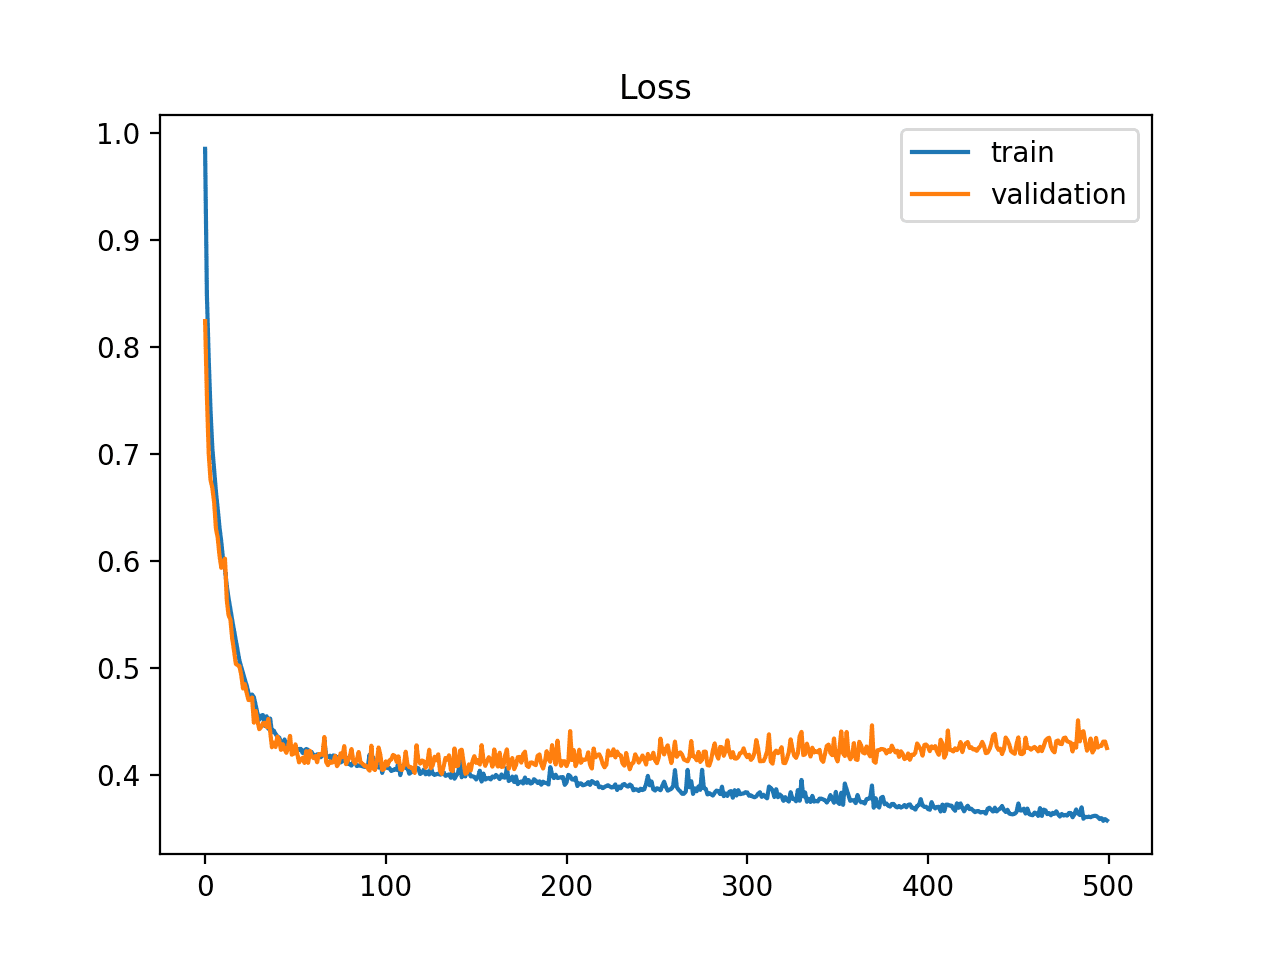
\includegraphics[width=.7\linewidth]{overfitting.png}
\end{center}
\end{frame}


\begin{frame}{Ранняя остановка}
\begin{center}
	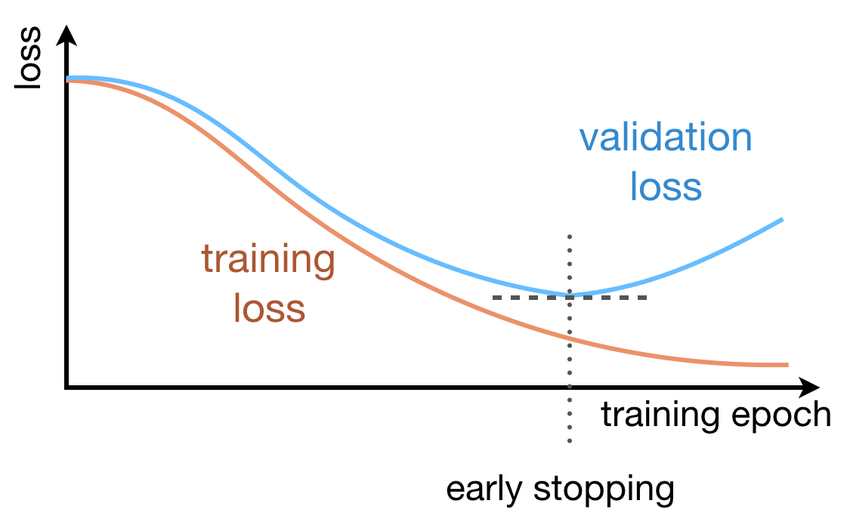
\includegraphics[width=.95\linewidth]{early_stopping.png}
\end{center}
\end{frame}


\begin{frame}{ }
\begin{center}
	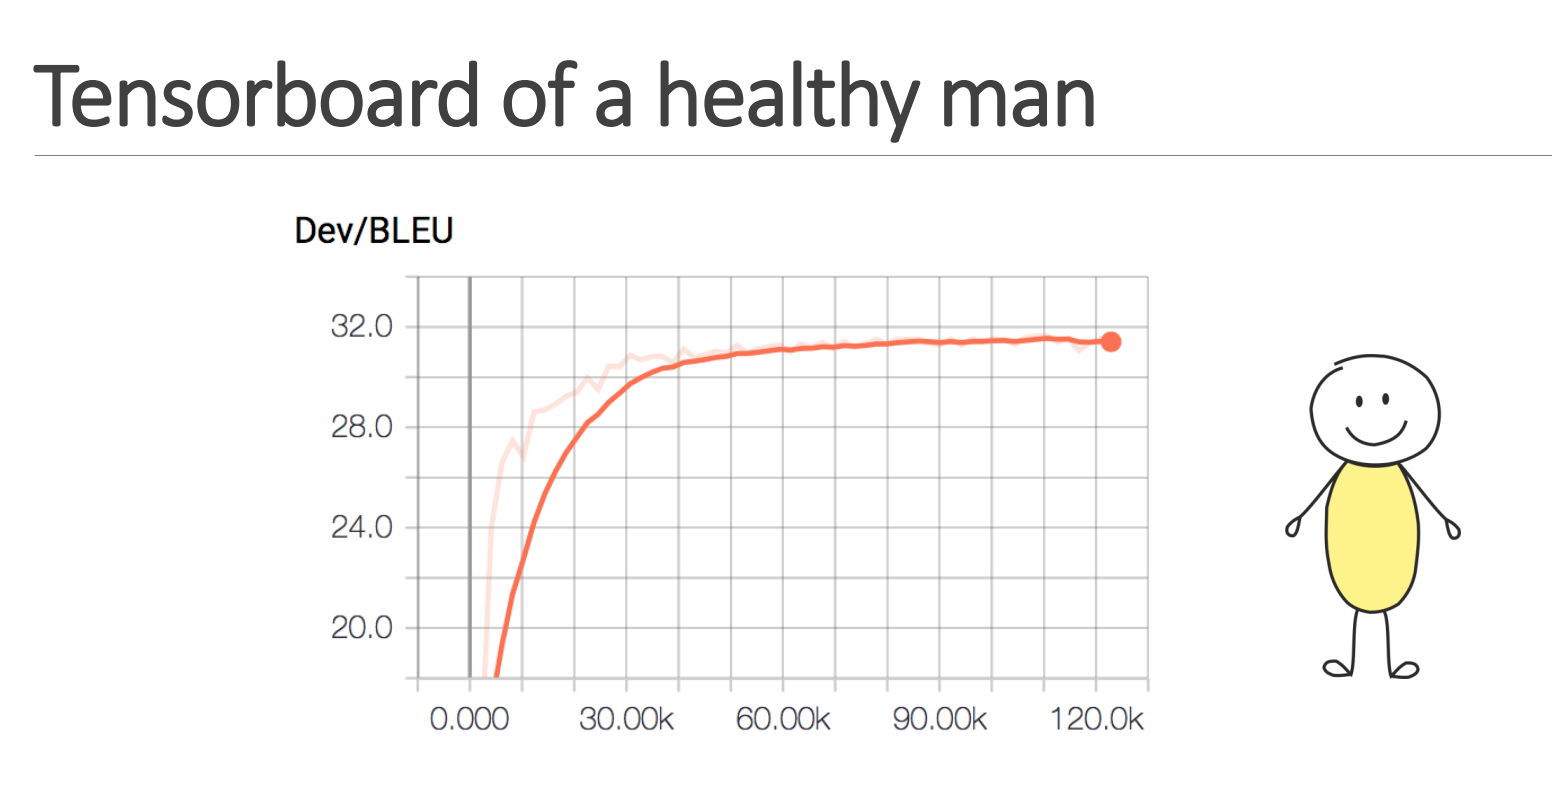
\includegraphics[width=.95\linewidth]{shuffle_1.png}
\end{center}
\vfill %
\footnotesize 
\color{blue} \url{https://github.com/yandexdataschool/nlp_course/tree/2019/week01_embeddings} \\ 
\url{https://lena-voita.github.io/nlp_course.html}
\end{frame}


\begin{frame}{ }
\begin{center}
	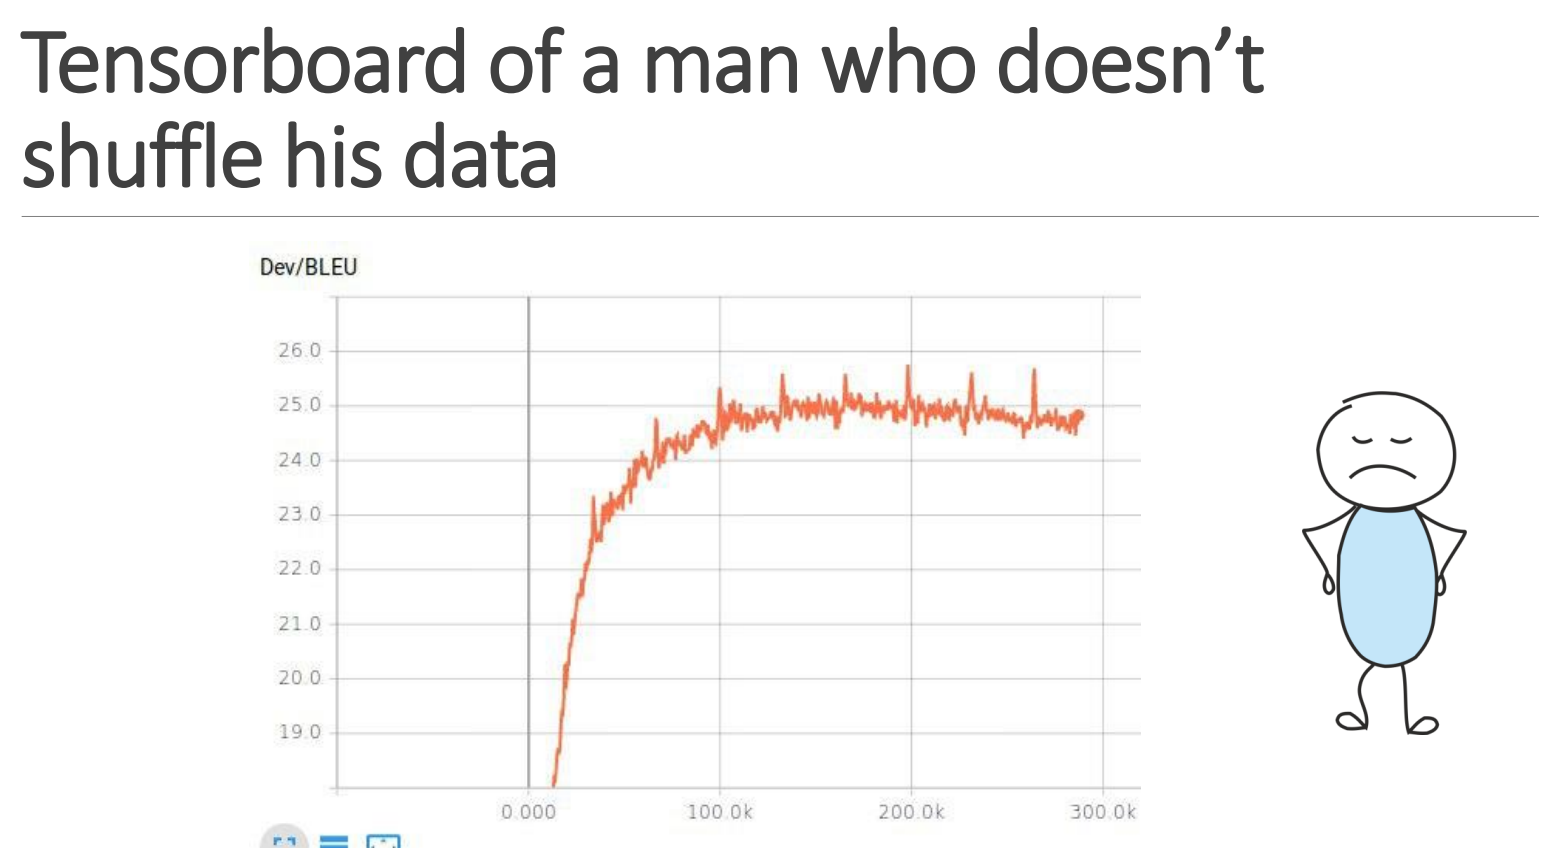
\includegraphics[width=.92\linewidth]{shuffle_2.png}
\end{center}
\vfill %
\footnotesize 
\color{blue} \url{https://github.com/yandexdataschool/nlp_course/tree/2019/week01_embeddings} \\
\url{https://lena-voita.github.io/nlp_course.html}
\end{frame}


\begin{frame}{ }
\begin{center}
	
\includegraphics[width=.9\linewidth]{shuffle_3.png}
\end{center}
\vfill %
\footnotesize 
\color{blue} \url{https://github.com/yandexdataschool/nlp_course/tree/2019/week01_embeddings} \\
\url{https://lena-voita.github.io/nlp_course.html}
\end{frame}



\begin{transitionframe}
	\begin{center}
		{\Huge Как обучить нейросеть?} \\ \mbox{ } \\
			\begin{tikzpicture}
			\node[inner sep=0pt] (russell) at (0,0)
			{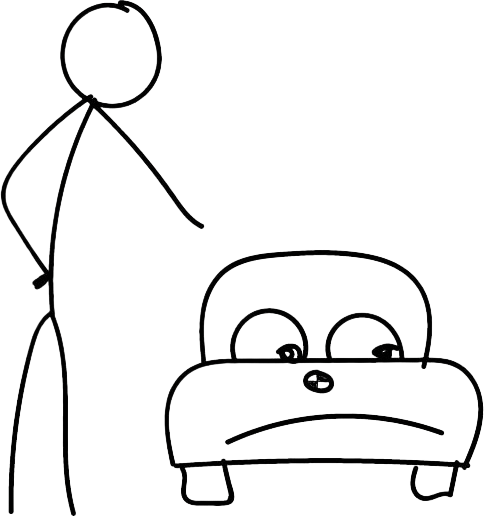
\includegraphics[scale = 0.15]{ml.png}};
			\node[] at (0,-0.6) {Ты необучаем!};
			\end{tikzpicture}
	\end{center}
\end{transitionframe}


\begin{frame}{Нейросеть —  сложная функция}
	\begin{wideitemize}
	\item Прямое распространение ошибки (forward propagation): 
	
	\[ X \Rightarrow X \cdot W_1 \Rightarrow f(X \cdot W_1) \Rightarrow f(X \cdot W_1) \cdot W_2 \Rightarrow \ldots \Rightarrow \hat{y} \]
	
	\item Считаем потери:
	
	\[Loss = \frac{1}{2} (y - \hat y)^2\]
	
	\item Все слои обычно дифференцируемы, поэтому можно посчитать производные по всем параметрам
	
	\item Для обучения можно использовать градиентный спуск
	\end{wideitemize}
\end{frame}


\begin{frame}{Как обучить нейросеть?}

\[ L(W_1, W_2) =  \frac{1}{2} \cdot (y - f(X \cdot W_1) \cdot W_2)^2\]

\begin{center}
\alert{Секрет успеха в умении брать производную}
\end{center}

\pause

\[ \boxed{ f(g(x))' = f'(g(x)) \cdot g'(x) }  \]

\pause

\begin{equation*} 
\begin{aligned} 
\frac{\partial L}{\partial W_2} &=   { \only<2>{ \color{red}} - (y - f(X \cdot W_1) \cdot W_2) } \cdot f(X \cdot W_1) \\
\frac{\partial L}{\partial W_1} &= { \only<2>{ \color{red}}  - (y - f(X \cdot W_1) \cdot W_2) } \cdot W_2 \cdot  f'(X \cdot W_1) \cdot X 
\end{aligned}
\end{equation*}

\vfill

\pause

\alert{Дважды ищем одно и то же $\Rightarrow$ оптимизация поиска производных даст нам алгоритм обратного распространения ошибки (back-propagation)}
\end{frame}


\begin{frame}{Back-propagation}
	\begin{center}
		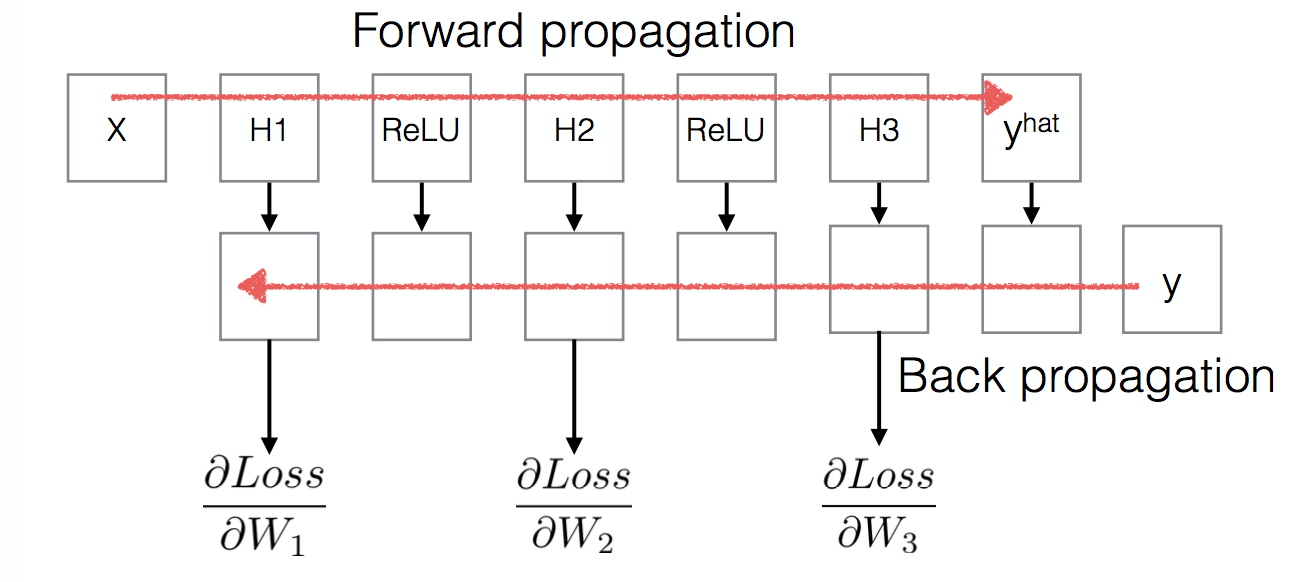
\includegraphics[width=.8\linewidth]{backpropagation.png}
	\end{center}
\end{frame}

%
%\begin{frame}{Цепное правило}
%	\begin{wideitemize}
%		\item  Возьмём сложную функцию: 
%		
%		\begin{equation*}
%		\begin{aligned}
%		& z_1 = z_1(x_1, x_2) \\  & z_2 = z_2(x_1, x_2) \\  & y = y(z_1, z_2)
%		\end{aligned}
%		\end{equation*} 
%		
%		\item Производную такой функции можно найти по цепному правилу: 
%		
%		$$
%		\frac{\partial y}{\partial x_1} = {\color{amethyst} \frac{\partial y}{\partial z_1}} \cdot {\color{red} \frac{\partial z_1}{\partial x_1}} + {\color{junglegreen} \frac{\partial y}{\partial z_2}} \cdot {\color{green} \frac{\partial z_2}{\partial x_1}}
%		$$ 
%	\end{wideitemize}
%\end{frame} 
%
%
%\begin{frame}{Как считать производные?}
%\begin{columns}
%	\begin{column}{0.6\textwidth}
%\begin{center}
%	\begin{tikzpicture}
%	\tikzstyle{place}=[circle, draw=black, minimum size = 8mm]
%	
%	% Input
%	\foreach \x in {1,...,2}
%	\draw node at (0, -\x*1.5) [place] (first_\x) {$x_\x$};
%	
%	% Hidden 1
%	\foreach \x in {1,...,2}
%	\node at (3, -\x*1.5) [place] (second_\x){$z_\x$};		
%		
%	% Output
%	\node at (6, -2.25) [place] (fourth){$y$};
%	
%	\draw [->, red]  (first_1) to (second_1);
%	\draw [->, green]  (first_1) to (second_2);
%	\draw [->]  (first_2) to (second_1);
%	\draw [->]  (first_2) to (second_2);
%	
%	\draw [->, amethyst]  (second_1) to (fourth);
%	\draw [->, junglegreen]  (second_2) to (fourth);
%	\end{tikzpicture}
%	\vfill
%	\begin{tikzpicture}
%	\tikzstyle{place}=[circle, draw=black, minimum size = 8mm]
%	
%	% Input
%	\foreach \x in {1,...,2}
%	\draw node at (0, -\x*1.5) [place] (second_\x) {$x_\x$};
%	
%	% Hidden 1
%	\foreach \x in {1,...,2}
%	\node at (3, -\x*1.5) [place] (first_\x){$z_\x$};		
%	
%	% Output
%	\node at (6, -2.25) [place] (fourth){$y$};
%	
%	\draw [->, dashed, red]  (first_1) to (second_1) node[right=1.cm] {$\frac{\partial z_1}{\partial x_1}$} ;
%	\draw [->, dashed]  (first_1) to (second_2) node[right=1.cm,above] {$\frac{\partial z_1}{\partial x_2}$} ;
%	\draw [->, dashed, green]  (first_2) to (second_1) node[right=2.3cm, below] {$\frac{\partial z_2}{\partial x_1}$} ;
%	\draw [->, dashed]  (first_2) to (second_2) node[right=1.2cm] {$\frac{\partial z_2}{\partial x_2}$} ;
%	
%	\draw [->, dashed, amethyst] (fourth)  to (first_1) node[right=1.cm] {$\frac{\partial y}{\partial z_1}$} ;
%	\draw [->, dashed, junglegreen] (fourth) to (first_2) node[right=1.cm] {$\frac{\partial y}{\partial z_2}$} ;
%	\end{tikzpicture}
%\end{center}
%\end{column}
%\begin{column}{0.4\textwidth}
%\textbf{Граф вычислений: }
%\begin{equation*} 
%\begin{aligned}
%	& z_1 = z_1(x_1, x_2)\\
%	& z_2 = z_2(x_1, x_2) \\
%	& y = y(z_1, z_2) 
%\end{aligned}
%\end{equation*} 
%\vfill 
%\only<1>{
%\alert{Из него можно построить граф производных, каждому ребру будет приписана производная}}
%
%\only<2>{\textbf{Можно догадаться как работает цепное правило:}
%	\[\frac{\partial y}{\partial x_1} = {\color{amethyst} \frac{\partial y}{\partial z_1}} \cdot {\color{red} \frac{\partial z_1}{\partial x_1}} + {\color{junglegreen} \frac{\partial y}{\partial z_2}} \cdot {\color{green} \frac{\partial z_2}{\partial x_1}} \]
%}
%\end{column}
%\end{columns}
%\end{frame} 
%
%
%
%\begin{frame}{Пойдём глубже}
%
%\begin{center}
%	\begin{tikzpicture}
%	\tikzstyle{place}=[circle, draw=black, minimum size = 8mm]
%	
%	% Input
%	\foreach \x in {1,...,2}
%	\draw node at (0, -\x*1.5) [place] (first_\x) {$x_\x$};
%	
%	% Hidden 1
%	\foreach \x in {1,...,2}
%	\node at (3, -\x*1.5) [place] (second_\x){$z_\x$};		
%	
%	% Hidden 2
%	\foreach \x in {1,...,2}
%	\node at (6, -\x*1.5) [place] (third_\x){$h_\x$};	
%	
%	% Output
%	\node at (9, -2.25) [place] (fourth){$y$};
%	
%	\draw [->, red]  (first_1) to (second_1);
%	\draw [->, green]  (first_1) to (second_2);
%	\draw [->, red]  (first_2) to (second_1);
%	\draw [->, green]  (first_2) to (second_2);
%	
%	\draw [->, amethyst]  (second_1) to (third_1);
%	\draw [->, junglegreen]  (second_1) to (third_2);
%	\draw [->, amethyst]  (second_2) to (third_1);
%	\draw [->, junglegreen]  (second_2) to (third_2);
%	
%	\draw [->, blue]  (third_1) to (fourth);
%	\draw [->, blue]  (third_2) to (fourth);
%
%	\end{tikzpicture}
%\end{center}
%
%\only<1>{
%\begin{equation*} 
%	\begin{aligned}
%		z_1 = z_1({\color{red} x_1, x_2})  & \quad   h_1 = h_1({\color{amethyst} z_1, z_2}) & \quad y = y({\color{blue} h_1, h_2}) \\
%		z_2 = z_2({\color{green} x_1, x_2}) & \quad h_2 = h_2({\color{junglegreen} z_1, z_2}) &  
%	\end{aligned}
%\end{equation*} }
%
%\only<2>{
%\[ \frac{\partial y}{\partial x_1} = ?  \]	
%}
%
%\only<3>{
%	\[ \frac{\partial y}{\partial x_1} = {\color{blue} \frac{\partial y}{\partial h_1}} \cdot  \frac{\partial h_1}{\partial x_1} + {\color{blue} \frac{\partial y}{\partial h_2}} \cdot \frac{\partial h_2}{\partial x_1}   \]	
%}
%
%\only<4>{
%	\[ \frac{\partial y}{\partial x_1} = {\color{blue} \frac{\partial y}{\partial h_1}} \cdot  \boxed{ \frac{\partial h_1}{\partial x_1}  } + {\color{blue} \frac{\partial y}{\partial h_2}} \cdot \boxed{ \frac{\partial h_2}{\partial x_1} }  \]	
%}
%
%\only<5>{
%	\[ \frac{\partial y}{\partial x_1} = {\color{blue} \frac{\partial y}{\partial h_1}} \cdot \underbrace{ \boxed{ \frac{\partial h_1}{\partial x_1}  }  }_{ {\color{amethyst} \frac{\partial h_1}{\partial z_1}} \cdot {\color{red} \frac{\partial z_1}{\partial x_1}} + {\color{amethyst} \frac{\partial h_1}{\partial z_2}} \cdot {\color{green} \frac{\partial z_2}{\partial x_1}}  }  + {\color{blue} \frac{\partial y}{\partial h_2}} \cdot \underbrace{\boxed{ \frac{\partial h_2}{\partial x_1} } }_{ {\color{junglegreen} \frac{\partial h_2}{\partial z_1}} \cdot {\color{red} \frac{\partial z_1}{\partial x_1}} + {\color{junglegreen} \frac{\partial h_2}{\partial z_2}} \cdot {\color{green} \frac{\partial z_2}{\partial x_1}}  } \]	
%}
%
%
%\only<6>{
%	\[ \frac{\partial y}{\partial x_1} = {\color{blue} \frac{\partial y}{\partial h_1}} \cdot \left( {\color{amethyst} \frac{\partial h_1}{\partial z_1}} \cdot {\color{red} \frac{\partial z_1}{\partial x_1}} + {\color{amethyst} \frac{\partial h_1}{\partial z_2}} \cdot {\color{green} \frac{\partial z_2}{\partial x_1}}  \right)  + {\color{blue} \frac{\partial y}{\partial h_2}} \cdot \left( {\color{junglegreen} \frac{\partial h_2}{\partial z_1}} \cdot {\color{red} \frac{\partial z_1}{\partial x_1}} + {\color{junglegreen} \frac{\partial h_2}{\partial z_2}} \cdot {\color{green} \frac{\partial z_2}{\partial x_1}}  \right) \]	
%}
%
%
%\only<7>{
%	\[ \frac{\partial y}{\partial x_1} = {\color{blue} \frac{\partial y}{\partial h_1}}  {\color{amethyst} \frac{\partial h_1}{\partial z_1}}  {\color{red} \frac{\partial z_1}{\partial x_1}}    +	{\color{blue} \frac{\partial y}{\partial h_1}}  {\color{amethyst} \frac{\partial h_1}{\partial z_2}}  {\color{green} \frac{\partial z_2}{\partial x_1}}  + {\color{blue} \frac{\partial y}{\partial h_2}}   {\color{junglegreen} \frac{\partial h_2}{\partial z_1}}  {\color{red} \frac{\partial z_1}{\partial x_1}} + {\color{blue} \frac{\partial y}{\partial h_2}}  {\color{junglegreen} \frac{\partial h_2}{\partial z_2}}  {\color{green} \frac{\partial z_2}{\partial x_1}}  \]	
%}
%
%\end{frame} 
%
%
%\begin{frame}{Пойдём глубже}
%
%\begin{center}
%	\begin{tikzpicture}
%	\tikzstyle{place}=[circle, draw=black, minimum size = 8mm]
%	
%	% Input
%	\foreach \x in {1,...,2}
%	\draw node at (0, -\x*1.5) [place] (first_\x) {$x_\x$};
%	
%	% Hidden 1
%	\foreach \x in {1,...,2}
%	\node at (3, -\x*1.5) [place] (second_\x){$z_\x$};		
%	
%	% Hidden 2
%	\foreach \x in {1,...,2}
%	\node at (6, -\x*1.5) [place] (third_\x){$h_\x$};	
%	
%	% Output
%	\node at (9, -2.25) [place] (fourth){$y$};
%		
%	\draw [->, dashed, red]  (second_1) to (first_1);
%	\draw [->, dashed, green]  (second_2) to (first_1);
%	\draw [->, dashed, red]  (second_1) to (first_2);
%	\draw [->, dashed, green]  (second_2) to (first_2);
%	
%	\draw [->, dashed, amethyst]  (third_1) to (second_1);
%	\draw [->, dashed, junglegreen]  (third_2) to (second_1);
%	\draw [->, dashed, amethyst] (third_1) to (second_2);
%	\draw [->, dashed, junglegreen]  (third_2) to (second_2);
%	
%	\draw [->, dashed,  blue]  (fourth) to (third_1);
%	\draw [->, dashed, blue]   (fourth) to (third_2);
%	
%	\only<2>{ 
%			\draw [->, dashed, ultra thick, blue]  (fourth) to (third_1);
%			\draw [->, dashed, ultra thick, amethyst]  (third_1) to (second_1);
%			\draw [->, dashed, ultra thick, red]  (second_1) to (first_1);
%	}
%
%	\only<3>{ 
%		\draw [->, dashed, ultra thick, blue]  (fourth) to (third_1);
%		\draw [->, dashed, ultra thick, amethyst]  (third_1) to (second_2);
%		\draw [->, dashed, ultra thick, green]  (second_2) to (first_1);
%	}
%
%	\only<4>{ 
%		\draw [->, dashed, ultra thick, blue]  (fourth) to (third_2);
%		\draw [->, dashed, ultra thick, junglegreen]  (third_2) to (second_1);
%		\draw [->, dashed, ultra thick, red]  (second_1) to (first_1);
%	}
%
%	\only<5>{ 
%		\draw [->, dashed, ultra thick, blue]  (fourth) to (third_2);
%		\draw [->, dashed, ultra thick, junglegreen]  (third_2) to (second_2);
%		\draw [->, dashed, ultra thick, green]  (second_2) to (first_1);
%	}
%	
%	\end{tikzpicture}
%\end{center}
%
%\only<1>{
%	\[ 
%	\frac{\partial y}{\partial x_1} = {\color{blue} \frac{\partial y}{\partial h_1}}  {\color{amethyst} \frac{\partial h_1}{\partial z_1}}  {\color{red} \frac{\partial z_1}{\partial x_1}}    +     {\color{blue} \frac{\partial y}{\partial h_1}}  {\color{amethyst} \frac{\partial h_1}{\partial z_2}}  {\color{green} \frac{\partial z_2}{\partial x_1}}     +       {\color{blue} \frac{\partial y}{\partial h_2}}   {\color{junglegreen} \frac{\partial h_2}{\partial z_1}}  {\color{red} \frac{\partial z_1}{\partial x_1}}      +      {\color{blue} \frac{\partial y}{\partial h_2}}  {\color{junglegreen} \frac{\partial h_2}{\partial z_2}}  {\color{green} \frac{\partial z_2}{\partial x_1}}  
%	\]	
%}
%
%\only<2>{
%	\[ 
%	\frac{\partial y}{\partial x_1} =  \boxed{ {\color{blue} \frac{\partial y}{\partial h_1}}  {\color{amethyst} \frac{\partial h_1}{\partial z_1}}  {\color{red} \frac{\partial z_1}{\partial x_1}} }   +     {\color{blue} \frac{\partial y}{\partial h_1}}  {\color{amethyst} \frac{\partial h_1}{\partial z_2}}  {\color{green} \frac{\partial z_2}{\partial x_1}}     +       {\color{blue} \frac{\partial y}{\partial h_2}}   {\color{junglegreen} \frac{\partial h_2}{\partial z_1}}  {\color{red} \frac{\partial z_1}{\partial x_1}}      +      {\color{blue} \frac{\partial y}{\partial h_2}}  {\color{junglegreen} \frac{\partial h_2}{\partial z_2}}  {\color{green} \frac{\partial z_2}{\partial x_1}}  
%	\]	
%}
%
%
%\only<3>{
%	\[ 
%	\frac{\partial y}{\partial x_1} = {\color{blue} \frac{\partial y}{\partial h_1}}  {\color{amethyst} \frac{\partial h_1}{\partial z_1}}  {\color{red} \frac{\partial z_1}{\partial x_1}}    +    \boxed{ {\color{blue} \frac{\partial y}{\partial h_1}}  {\color{amethyst} \frac{\partial h_1}{\partial z_2}}  {\color{green} \frac{\partial z_2}{\partial x_1}} }    +       {\color{blue} \frac{\partial y}{\partial h_2}}   {\color{junglegreen} \frac{\partial h_2}{\partial z_1}}  {\color{red} \frac{\partial z_1}{\partial x_1}}      +      {\color{blue} \frac{\partial y}{\partial h_2}}  {\color{junglegreen} \frac{\partial h_2}{\partial z_2}}  {\color{green} \frac{\partial z_2}{\partial x_1}}  
%	\]	
%}
%
%\only<4>{
%	\[ 
%	\frac{\partial y}{\partial x_1} = {\color{blue} \frac{\partial y}{\partial h_1}}  {\color{amethyst} \frac{\partial h_1}{\partial z_1}}  {\color{red} \frac{\partial z_1}{\partial x_1}}    +     {\color{blue} \frac{\partial y}{\partial h_1}}  {\color{amethyst} \frac{\partial h_1}{\partial z_2}}  {\color{green} \frac{\partial z_2}{\partial x_1}}     +      \boxed{ {\color{blue} \frac{\partial y}{\partial h_2}}   {\color{junglegreen} \frac{\partial h_2}{\partial z_1}}  {\color{red} \frac{\partial z_1}{\partial x_1}} }     +      {\color{blue} \frac{\partial y}{\partial h_2}}  {\color{junglegreen} \frac{\partial h_2}{\partial z_2}}  {\color{green} \frac{\partial z_2}{\partial x_1}}  
%	\]	
%}
%
%\only<5>{
%	\[ 
%	\frac{\partial y}{\partial x_1} = {\color{blue} \frac{\partial y}{\partial h_1}}  {\color{amethyst} \frac{\partial h_1}{\partial z_1}}  {\color{red} \frac{\partial z_1}{\partial x_1}}    +     {\color{blue} \frac{\partial y}{\partial h_1}}  {\color{amethyst} \frac{\partial h_1}{\partial z_2}}  {\color{green} \frac{\partial z_2}{\partial x_1}}     +       {\color{blue} \frac{\partial y}{\partial h_2}}   {\color{junglegreen} \frac{\partial h_2}{\partial z_1}}  {\color{red} \frac{\partial z_1}{\partial x_1}}      +    \boxed{  {\color{blue} \frac{\partial y}{\partial h_2}}  {\color{junglegreen} \frac{\partial h_2}{\partial z_2}}  {\color{green} \frac{\partial z_2}{\partial x_1}}  }
%	\]	
%}
%
%\end{frame} 
%
%
%\begin{frame}{Алгоритм поиска производной в графе}
%	\begin{wideitemize}
%		\item Как посчитать производную $a$ по $b$? 
%		
%		\item Находим непосещённый путь из $a$ в $b$ 
%		
%		\item Перемножаем значения на рёбрах пути 
%		
%		\item Добавляем в сумму
%		
%	\end{wideitemize}	
%\vspace{-1.5cm}
%\begin{columns}
%\begin{column}{0.4\textwidth}
%\begin{center}
%\begin{tikzpicture}
%\tikzstyle{place}=[circle, draw=black, minimum size = 8mm]
%
%% Input
%\foreach \x in {1,...,2}
%\draw node at (0, -\x*1.5) [place] (second_\x) {$x_\x$};
%
%% Hidden 1
%\foreach \x in {1,...,2}
%\node at (3, -\x*1.5) [place] (first_\x){$z_\x$};		
%
%% Output
%\node at (6, -2.25) [place] (fourth){$y$};
%
%\draw [->, dashed, red]  (first_1) to (second_1) node[right=1.cm] {$\frac{\partial z_1}{\partial x_1}$} ;
%\draw [->, dashed]  (first_1) to (second_2);
%\draw [->, dashed, green]  (first_2) to (second_1) node[right=2.3cm, below] {$\frac{\partial z_2}{\partial x_1}$} ;
%\draw [->, dashed]  (first_2) to (second_2); 
%
%\draw [->, dashed, amethyst] (fourth)  to (first_1) node[right=1.cm] {$\frac{\partial y}{\partial z_1}$} ;
%\draw [->, dashed, junglegreen] (fourth) to (first_2) node[right=1.cm] {$\frac{\partial y}{\partial z_2}$} ;
%\end{tikzpicture}
%\end{center}
%\end{column}
%\begin{column}{0.4\textwidth}
%\[ 
%\frac{\partial y}{\partial x_1} =  {\color{amethyst} \frac{\partial y}{\partial z_1} } \cdot {\color{red}  \frac{\partial z_1}{\partial x_1} } + {\color{ junglegreen}  \frac{\partial y}{\partial z_2} } \cdot {\color{green} \frac{\partial z_2}{\partial x_1 } }
%\]
%\end{column}
%\end{columns}
%\end{frame}
%
%
%\begin{frame}{На примере одного нейрона}
%\begin{center}
%	\begin{tikzpicture}
%		\tikzstyle{place}=[circle, draw=black, minimum size = 8mm]
%		
%		% Input
%		\foreach \x in {1,...,2}
%		\draw node at (0, -\x*1.5) [place] (first_\x) {$x_\x$};
%		
%		% weights
%		\draw node at (1, -0.5) [place] (param_1) {$w_1$};
%		\draw node at (1, -4) [place] (param_2) {$w_2$};
%		
%		% product
%		\foreach \x in {1,...,2}
%		\node at (3, -\x*1.5) [place] (second_\x){$\cdot$};		
%
%		% sum
%		\node at (5, -2.25) [place] (sum){$s$};
%		\node at (7, -2.25) [place] (activ){$f$};
%		\node at (9, -2.25) [place] (out){$z$};
%		\node at (11, -2.75) [place] (loss){$L$};
%		\node at (9, -3.25) [place] (target){$y$};
%		
%		\draw [->]  (first_1) to (second_1);
%		\draw [->]  (first_2) to (second_2);	
%		\draw [->]  (param_1) to (second_1);
%		\draw [->]  (param_2) to (second_2);
%		
%		\draw [->] (second_1) to (sum);
%		\draw [->] (second_2) to (sum);
%		
%		\draw [->] (sum) to (activ);
%		\draw [->] (activ) to (out);
%		\draw [->] (out) to (loss);
%		\draw [->] (target) to (loss);
%	\end{tikzpicture}
%
%	
%	\begin{equation*}
%			z = f(s) = f(w_1 \cdot x_1 + w_2 \cdot x_2)
%	\end{equation*}
%	
%	\alert{ Для SGD нам нужны $\frac{\partial L}{\partial w_1}$  и $\frac{\partial L}{\partial w_2}$ }
%\end{center}
%\end{frame}	
%
%
%
%\begin{frame}{Граф производных}
%\begin{center}
%	\begin{tikzpicture}
%	\tikzstyle{place}=[circle, draw=black, minimum size = 8mm]
%	
%	% Input
%	\foreach \x in {1,...,2}
%	\draw node at (0, -\x*1.5) [place] (first_\x) {$x_\x$};
%	
%	% weights
%	\draw node at (1, -0.5) [place] (param_1) {$w_1$};
%	\draw node at (1, -4) [place] (param_2) {$w_2$};
%	
%	% product
%	\foreach \x in {1,...,2}
%	\node at (3, -\x*1.5) [place] (second_\x){$\cdot$};		
%	
%	% sum
%	\node at (5, -2.25) [place] (sum){$s$};
%	\node at (7, -2.25) [place] (activ){$f$};
%	\node at (9, -2.25) [place] (out){$z$};
%	\node at (11, -2.75) [place] (loss){$L$};
%	\node at (9, -3.25) [place] (target){$y$};
%	
%	\only<1>{
%	\draw [->, dashed, red]  (second_1) to (first_1) node[below right=2.mm] {$w_1$} ;
%	\draw [->, dashed, red]  (second_2) to (first_2) node[above right=2.mm] {$w_2$} ;
%	\draw [->, dashed, red]  (second_1) to (param_1) node[right=1.cm] {$x_1$} ;
%	\draw [->, dashed, red]  (second_2) to (param_2) node[right=1.cm] {$x_2$} ;
%	
%	\draw [->, dashed, red] (sum) to (second_1)  node[right=8.mm] {$1$} ;
%	\draw [->, dashed, red] (sum) to (second_2)  node[right=8.mm] {$1$} ;
%	
%	\draw [->, dashed, red] (activ) to (sum)  node[right=6.mm] {$\frac{\partial f}{\partial s}$} ;
%	\draw [->, dashed, red] (out) to (activ)  node[right=7.mm] {$1$} ;
%	\draw [->, dashed] (loss) to (out) node[right=7.mm] {$\frac{\partial L}{\partial z}$} ;
%	\draw [->, dashed] (loss) to (target) ;
%	}
%
%	\only<2>{
%	\draw [->, dashed, red]  (second_1) to (first_1) node[below right=2.mm] {$w_1$} ;
%	\draw [->, dashed, red]  (second_2) to (first_2) node[above right=2.mm] {$w_2$} ;
%	\draw [->, dashed, amethyst, ultra thick]  (second_1) to (param_1) node[right=1.cm] {$x_1$} ;
%	\draw [->, dashed, red]  (second_2) to (param_2) node[right=1.cm] {$x_2$} ;
%	
%	\draw [->, dashed, amethyst, ultra thick] (sum) to (second_1)  node[right=8.mm] {$1$} ;
%	\draw [->, dashed, red] (sum) to (second_2)  node[right=8.mm] {$1$} ;
%	
%	\draw [->, dashed, amethyst, ultra thick] (activ) to (sum)  node[right=6.mm] {$\frac{\partial f}{\partial s}$} ;
%	\draw [->, dashed, amethyst, ultra thick] (out) to (activ)  node[right=7.mm] {$1$} ;
%	\draw [->, dashed, amethyst, ultra thick] (loss) to (out) node[right=7.mm] {$\frac{\partial L}{\partial z}$} ;
%	\draw [->, dashed] (loss) to (target) ;
%	}
%
%	\only<3>{
%	\draw [->, dashed, red]  (second_1) to (first_1) node[below right=2.mm] {$w_1$} ;
%	\draw [->, dashed, red]  (second_2) to (first_2) node[above right=2.mm] {$w_2$} ;
%	\draw [->, dashed, red]  (second_1) to (param_1) node[right=1.cm] {$x_1$} ;
%	\draw [->, dashed, amethyst,  ultra thick]  (second_2) to (param_2) node[right=1.cm] {$x_2$} ;
%	
%	\draw [->, dashed, red] (sum) to (second_1)  node[right=8.mm] {$1$} ;
%	\draw [->, dashed, amethyst, ultra thick] (sum) to (second_2)  node[right=8.mm] {$1$} ;
%	
%	\draw [->, dashed, amethyst, ultra thick] (activ) to (sum)  node[right=6.mm] {$\frac{\partial f}{\partial s}$} ;
%	\draw [->, dashed, amethyst, ultra thick] (out) to (activ)  node[right=7.mm] {$1$} ;
%	\draw [->, dashed, amethyst, ultra thick] (loss) to (out) node[right=7.mm] {$\frac{\partial L}{\partial z}$} ;
%	\draw [->, dashed] (loss) to (target) ;
%	}
%
%	\end{tikzpicture}
%
%	\begin{equation*}
%	z = f(s) = f(w_1 \cdot x_1 + w_2 \cdot x_2)
%	\end{equation*}
%	
%	\only<1> { \alert{ Для SGD нам нужны $\frac{\partial L}{\partial w_1}$  и $\frac{\partial L}{\partial w_2}$ } }
%	
%	\only<2>{ 
%	\[
%		\frac{\partial L}{\partial w_1} = \frac{\partial L}{\partial z} \cdot \frac{\partial f}{\partial s} \cdot x_1 
%	\] }
%
%	\only<3>{ 
%	\[
%		\frac{\partial L}{\partial w_1} = \frac{\partial L}{\partial z} \cdot \frac{\partial f}{\partial s} \cdot x_1  \qquad  \frac{\partial L}{\partial w_2} = \frac{\partial L}{\partial z} \cdot \frac{\partial f}{\partial s} \cdot x_2  
%	\] }
%\end{center}
%\end{frame}	
%
%
%\begin{frame}{Цепное правило и грaф производных}
%\begin{wideitemize} 
%	\item Теперь у нас есть алгоритм для подсчета производных для любых
%	дифференцируемых графов вычислений
%	
%	\item \alert{ Осталось делать вычисления быстро }
%\end{wideitemize} 
%\end{frame}
%
%
%
%\begin{frame}{Обратное распространение ошибки}
%
%\alert{Мы хотим поменять параметры нейрона в рамках SGD}
%
%\vfill
%
%\[
%h_2 = f(w_0 + w_1 z_1 + w_2 z_2)
%\]
%
%\vfill
%
%\[
%\frac{\partial L}{\partial w_1} = \frac{\partial L}{\partial y} \cdot \frac{\partial y}{\partial w_1} =  \frac{\partial L}{\partial y} \cdot {\color{blue} \frac{\partial y}{\partial h_2}} \cdot \frac{\partial h_2}{\partial w_1} 
%\]
%
%\vfill
%
%\[
%w_1^t = w_1^{t-1} - \gamma \cdot \frac{\partial L}{\partial w_1} (w_1^{t-1})
%\]
%\end{frame}
%
%
%\begin{frame}{Обратное распространение ошибки}
%\begin{equation*} 
%\begin{aligned}
%	\only<1-6>{ & 3: \quad  {\color{blue} \frac{\partial y}{\partial h_2} \qquad \frac{\partial y}{\partial h_1}} \\} 
%	\only<2-6>{& 2: \quad \frac{\partial y}{\partial z_1} = {\color{blue} \frac{\partial y}{\partial h_1}} \cdot {\color{amethyst} \frac{\partial h_1}{\partial z_1}} + \frac{\partial y}{\partial h_2} \cdot {\color{junglegreen} \frac{\partial h_2}{\partial z_1}}   \qquad  \frac{\partial y}{\partial z_2} =  {\color{blue} \frac{\partial y}{\partial h_1}} \cdot {\color{amethyst} \frac{\partial h_1}{\partial z_2}}  + {\color{blue} \frac{\partial y}{\partial h_2}} \cdot {\color{junglegreen} \frac{\partial h_2}{\partial z_2}} \\} 
%	\only<3>{& 1: \quad \frac{\partial y}{\partial x_1} = {\color{blue} \frac{\partial y}{\partial h_1}}  {\color{amethyst} \frac{\partial h_1}{\partial z_1}}  {\color{red} \frac{\partial z_1}{\partial x_1}}    +    {\color{blue} \frac{\partial y}{\partial h_2}}   {\color{junglegreen} \frac{\partial h_2}{\partial z_1}}  {\color{red} \frac{\partial z_1}{\partial x_1}}      +  {\color{blue} \frac{\partial y}{\partial h_1}}  {\color{amethyst} \frac{\partial h_1}{\partial z_2}}  {\color{green} \frac{\partial z_2}{\partial x_1}}     +             {\color{blue} \frac{\partial y}{\partial h_2}}  {\color{junglegreen} \frac{\partial h_2}{\partial z_2}}  {\color{green} \frac{\partial z_2}{\partial x_1}} \\ }  
%	\only<4>{& 1: \quad \frac{\partial y}{\partial x_1} = \left( {\color{blue} \frac{\partial y}{\partial h_1}}  {\color{amethyst} \frac{\partial h_1}{\partial z_1}}    + {\color{blue} \frac{\partial y}{\partial h_2}}   {\color{junglegreen} \frac{\partial h_2}{\partial z_1}}  \right) \cdot {\color{red} \frac{\partial z_1}{\partial x_1}}  + \left( {\color{blue} \frac{\partial y}{\partial h_1}}  {\color{amethyst} \frac{\partial h_1}{\partial z_2}} +    {\color{blue} \frac{\partial y}{\partial h_2}}  {\color{junglegreen} \frac{\partial h_2}{\partial z_2}}  \right) \cdot {\color{green} \frac{\partial z_2}{\partial x_1}} \\  }
%	\only<5>{& 1: \quad \frac{\partial y}{\partial x_1} =  \frac{\partial y}{\partial z_1} \cdot {\color{red} \frac{\partial z_1}{\partial x_1}}  + \frac{\partial y}{\partial z_2} \cdot {\color{green} \frac{\partial z_2}{\partial x_1}} \\  }
%	\only<6>{& 1: \quad \frac{\partial y}{\partial x_1} =  \frac{\partial y}{\partial z_1} \cdot {\color{red} \frac{\partial z_1}{\partial x_1}}  + \frac{\partial y}{\partial z_2} \cdot {\color{green} \frac{\partial z_2}{\partial x_1}} \qquad \frac{\partial y}{\partial x_2} =  \frac{\partial y}{\partial z_1} \cdot {\color{red} \frac{\partial z_1}{\partial x_2}}  + \frac{\partial y}{\partial z_2} \cdot {\color{green} \frac{\partial z_2}{\partial x_2}}  \\  }
%	\only<7>{
%		& 3: \quad  {\color{blue} \frac{\partial y}{\partial h_2}   \qquad  \boxed{ \frac{\partial y}{\partial h_1}} } \\
%		& 2: \quad \boxed{ \frac{\partial y}{\partial z_1} } = {\color{blue}   \boxed{  \frac{\partial y}{\partial h_1}}}  \cdot {\color{amethyst} \frac{\partial h_1}{\partial z_1}} + \frac{\partial y}{\partial h_2} \cdot {\color{junglegreen} \frac{\partial h_2}{\partial z_2}}   \qquad  \frac{\partial y}{\partial z_2} =  {\color{blue} \boxed{ \frac{\partial y}{\partial h_1}} } \cdot {\color{amethyst} \frac{\partial h_1}{\partial z_2}}  + {\color{blue} \frac{\partial y}{\partial h_2}} \cdot {\color{junglegreen} \frac{\partial h_2}{\partial z_2}} \\
%		& 1: \quad \frac{\partial y}{\partial x_1} =  \boxed{ \frac{\partial y}{\partial z_1} } \cdot {\color{red} \frac{\partial z_1}{\partial x_1}}  + \frac{\partial y}{\partial z_2} \cdot {\color{green} \frac{\partial z_2}{\partial x_1}} \qquad \frac{\partial y}{\partial x_2} = \boxed{ \frac{\partial y}{\partial z_1}} \cdot {\color{red} \frac{\partial z_1}{\partial x_2}}  + \frac{\partial y}{\partial z_2} \cdot {\color{green} \frac{\partial z_2}{\partial x_2}}  \\  
%	}
%\end{aligned} 
%\end{equation*}
%
%\begin{center}
%	\begin{tikzpicture}
%	\tikzstyle{place}=[circle, draw=black, minimum size = 8mm]
%	
%	% Input
%	\foreach \x in {1,...,2}
%	\draw node at (0, -\x*1.5) [place] (first_\x) {$x_\x$};
%	
%	% Hidden 1
%	\foreach \x in {1,...,2}
%	\node at (3, -\x*1.5) [place] (second_\x){$z_\x$};		
%	
%	% Hidden 2
%	\foreach \x in {1,...,2}
%	\node at (6, -\x*1.5) [place] (third_\x){$h_\x$};	
%	
%	% Output
%	\node at (9, -2.25) [place] (fourth){$y$};
%	
%	\draw [->, dashed, red]  (second_1) to (first_1);
%	\draw [->, dashed, green]  (second_2) to (first_1);
%	\draw [->, dashed, red]  (second_1) to (first_2);
%	\draw [->, dashed, green]  (second_2) to (first_2);
%	
%	\draw [->, dashed, amethyst]  (third_1) to (second_1);
%	\draw [->, dashed, junglegreen]  (third_2) to (second_1);
%	\draw [->, dashed, amethyst] (third_1) to (second_2);
%	\draw [->, dashed, junglegreen]  (third_2) to (second_2);
%	
%	\draw [->, dashed,  blue]  (fourth) to (third_1);
%	\draw [->, dashed, blue]   (fourth) to (third_2);
%	
%	\only<1-6>{ 
%		\draw [->, dashed,  ultra thick, blue]  (fourth) to (third_1);
%		\draw [->, dashed, ultra thick, blue]   (fourth) to (third_2);
%	}
%
%	\only<2-6>{ 
%		\draw [->, dashed, ultra thick, amethyst]  (third_1) to (second_1);
%		\draw [->, dashed, ultra thick, junglegreen]  (third_2) to (second_1);
%	}
%
%	\only<3-6>{ 
%		\draw [->, dashed, ultra thick, red]  (second_1) to (first_1);
%	}
%	\end{tikzpicture}
%\end{center}
%\end{frame}
%
%
%\begin{frame}{Обратное распространение ошибки}
%\begin{wideitemize} 
%	\item Это называется reverse-mode дифференцирование, в теории нейросетей это называют \alert{back-propagation (обратное распространение ошибки)}
%	
%	\item Работает быстро, потому что переиспользует вычисленные ранее значения
%	
%	\item На самом деле, по каждому ребру пройдемся всего раз, то есть сложность линейна	по количеству ребер (т.е. параметров)
%\end{wideitemize} 
%\end{frame}
%
%
%\begin{frame}{Back-propagation на одном нейроне}
%\begin{center}
%	\begin{tikzpicture}
%	\tikzstyle{place}=[circle, draw=black, minimum size = 8mm]
%	\tikzstyle{place2}=[circle, draw=red, minimum size = 8mm]
%	
%	% Input
%	\foreach \x in {1,...,2}
%	\draw node at (0, -\x*1.5) [place] (first_\x) {$x_\x$};
%	
%	% weights
%	\draw node at (1, -0.5) [place] (param_1) {$w_1$};
%	\draw node at (1, -4) [place] (param_2) {$w_2$};
%	
%	% product
%	\foreach \x in {1,...,2}
%	\node at (3, -\x*1.5) [place] (second_\x){$\cdot$};		
%	
%	\node[thick] at (7, -1) {$z = \sigma(s) = \sigma(w_1 x_1 + w_2 x_2)$};
%	
%	% sum
%	\node  at (5, -2.25) [place] (sum){$s$};
%	\node at (7, -2.25) [place] (activ){$\sigma$};
%	\node at (9, -2.25) [place] (out){$z$};
%	
%	\draw [->]  (first_1) to (second_1);
%	\draw [->]  (first_2) to (second_2);	
%	\draw [->]  (param_1) to (second_1);
%	\draw [->]  (param_2) to (second_2);
%	
%	\draw [->] (second_1) to (sum);
%	\draw [->] (second_2) to (sum);
%	
%	\draw [->] (sum) to (activ);
%	\draw [->] (activ) to (out);
%\end{tikzpicture}
%\end{center}
%	
%\vfill 
%	
%Данные текут сквозь нейрон:
%
%\[  \boxed{X} \Rightarrow \boxed{s = X \cdot W}  \Rightarrow  \boxed{z =\sigma(s)}   \Rightarrow  \boxed{L(z, y) = (y - z)^2 }\]
%\end{frame} 
%
%
%\begin{frame}{Back-propagation на одном нейроне}
%
%Forward pass:
%
%\only<1>{ \[  \boxed{X} \Rightarrow \boxed{s = X \cdot W}  \Rightarrow  \boxed{z =\sigma(s)}   \Rightarrow  \boxed{L(z, y) = (y - z)^2 }\] }
%
%\only<2>{ \[  \boxed{X} \Rightarrow { \color{amethyst} \boxed{s = X \cdot W} }  \Rightarrow  \boxed{z =\sigma(s)}   \Rightarrow  \boxed{L(z, y) = (y - z)^2 }\] }
%
%Backward pass: 
%
%\begin{center}
%	\begin{tikzpicture}
%	\tikzstyle{place}=[circle, draw=black, minimum size = 8mm]
%	
%	% Input
%	\foreach \x in {1,...,2}
%	\draw node at (0, -\x*1.5) [place] (first_\x) {$x_\x$};
%	
%	% weights
%	\draw node at (1, -0.5) [place] (param_1) {$w_1$};
%	\draw node at (1, -4) [place] (param_2) {$w_2$};
%	
%	% product
%	\foreach \x in {1,...,2}
%	\node at (3, -\x*1.5) [place] (second_\x){$\cdot$};		
%	
%	% sum
%	\node at (5, -2.25) [place] (sum){$s$};
%	\node at (7, -2.25) [place] (activ){$f$};
%	\node at (9, -2.25) [place] (out){$z$};
%	\node at (11, -2.75) [place] (loss){$L$};
%	\node at (9, -3.25) [place] (target){$y$};
%	
%	\only<2>{
%		\node[amethyst,  thick] at (7, 0.4) {\text{Нам нужно вычислить} };
%		\node[amethyst,  thick] at (7, 0) {\text{сигмоиду в точке s} };
%		
%		\node[thick] at (8, -1) {$\frac{\partial \sigma}{\partial s} = \sigma(s) \cdot (1 - \sigma(s))$};
%	}
%	
%	\draw [->, dashed, red]  (second_1) to (first_1) node[below right=2.mm] {$w_1$} ;
%	\draw [->, dashed, red]  (second_2) to (first_2) node[above right=2.mm] {$w_2$} ;
%	\draw [->, dashed, red]  (second_1) to (param_1) node[right=1.cm] {$x_1$} ;
%	\draw [->, dashed, red]  (second_2) to (param_2) node[right=1.cm] {$x_2$} ;
%	
%	\draw [->, dashed, red] (sum) to (second_1)  node[right=8.mm] {$1$} ;
%	\draw [->, dashed, red] (sum) to (second_2)  node[right=8.mm] {$1$} ;
%	
%	\only<1>{ \draw [->, dashed, red] (activ) to (sum)  node[right=6.mm] {$\frac{\partial \sigma}{\partial s}$} ; }
%	
%	\only<2>{ \draw [->, dashed, ultra thick, amethyst] (activ) to (sum)  node[right=6.mm] {$\frac{\partial \sigma}{\partial s}$} ; }
%	
%	\draw [->, dashed, red] (out) to (activ)  node[right=7.mm] {$1$} ;
%	\draw [->, dashed] (loss) to (out) node[right=7.mm] {$\frac{\partial L}{\partial z}$} ;
%	\draw [->, dashed] (loss) to (target) ;
%	\end{tikzpicture}
%\end{center}
%\end{frame} 
%
%
%\begin{frame}{Сигмоида: прямой проход (forward pass)}
%\begin{center}
%	\begin{tikzpicture}
%	\tikzstyle{place}=[circle, draw=black, minimum size = 8mm]
%	\tikzstyle{place2}=[circle, draw=red, minimum size = 8mm]
%	
%	% Input
%	\foreach \x in {1,...,2}
%	\draw node at (0, -\x*1.5) [place] (first_\x) {$x_\x$};
%	
%	% weights
%	\draw node at (1, -0.5) [place] (param_1) {$w_1$};
%	\draw node at (1, -4) [place] (param_2) {$w_2$};
%	
%	% product
%	\foreach \x in {1,...,2}
%	\node at (3, -\x*1.5) [place] (second_\x){$\cdot$};		
%	
%	\node[thick] at (7, -1) {$z = \sigma(s) = \sigma(w_1 x_1 + w_2 x_2)$};
%	
%	% sum
%	\node  at (5, -2.25) [place2] (sum){\color{red} $s$};
%	\node at (7, -2.25) [place2] (activ){\color{red} $\sigma$};
%	\node at (9, -2.25) [place2] (out){\color{red} $z$};
%	
%	\draw [->]  (first_1) to (second_1);
%	\draw [->]  (first_2) to (second_2);	
%	\draw [->]  (param_1) to (second_1);
%	\draw [->]  (param_2) to (second_2);
%	
%	\draw [->] (second_1) to (sum);
%	\draw [->] (second_2) to (sum);
%	
%	\draw [->, red] (sum) to (activ);
%	\draw [->, red] (activ) to (out);
%	\end{tikzpicture}
%\end{center}
%	
%{\color{green} def}  {\color{blue} forward\_pass}(s):  \\
%\mbox{ } \hspace{5mm} {\color{green} return } 1/(1 + np.exp(-s))
%\end{frame} 
%
%
%
%\begin{frame}{Сигмоида: обратный проход (backward pass)}
%\begin{center}
%	\begin{tikzpicture}
%	\tikzstyle{place}=[circle, draw=black, minimum size = 8mm]
%	\tikzstyle{place2}=[circle, draw=red, minimum size = 8mm]
%	\tikzstyle{place3}=[circle, draw=amethyst, minimum size = 8mm]
%	
%	% Input
%	\foreach \x in {1,...,2}
%	\draw node at (0, -\x*1.5) [place] (first_\x) {$x_\x$};
%	
%	% weights
%	\draw node at (1, -0.5) [place] (param_1) {$w_1$};
%	\draw node at (1, -4) [place] (param_2) {$w_2$};
%	
%	% product
%	\foreach \x in {1,...,2}
%	\node at (3, -\x*1.5) [place] (second_\x){$\cdot$};		
%	
%	% sum
%	\node at (5, -2.25) [place3] (sum){\color{amethyst} $s$};
%	\node at (7, -2.25) [place2] (activ){\color{red} $\sigma$};
%	\node at (9, -2.25) [place2] (out){\color{red} $z$};
%	\node at (11, -2.75) [place] (loss){$L$};
%	\node at (9, -3.25) [place] (target){$y$};
%	
%	\node[amethyst,  thick] at (7, 0.4) {\text{Нам нужно вычислить} };
%	\node[amethyst,  thick] at (7, 0) {\text{сигмоиду в точке s} };
%	
%	\node[thick] at (8, -1) {\color{red} $\frac{\partial \sigma}{\partial s} = \sigma(s) \cdot (1 - \sigma(s))$};
%	
%	\draw [->, dashed]  (second_1) to (first_1) node[below right=2.mm] {$w_1$} ;
%	\draw [->, dashed]  (second_2) to (first_2) node[above right=2.mm] {$w_2$} ;
%	\draw [->, dashed]  (second_1) to (param_1) node[right=1.cm] {$x_1$} ;
%	\draw [->, dashed]  (second_2) to (param_2) node[right=1.cm] {$x_2$} ;
%	
%	\draw [->, dashed] (sum) to (second_1)  node[right=8.mm] {$1$} ;
%	\draw [->, dashed] (sum) to (second_2)  node[right=8.mm] {$1$} ;
%	
%	 \draw [->, dashed, red] (activ) to (sum)  node[right=6.mm] {$\frac{\partial \sigma}{\partial s}$} ; 
%	
%	\draw [->, dashed, red] (out) to (activ)  node[right=7.mm] {$1$} ;
%	\draw [->, dashed, junglegreen] (loss) to (out) node[right=7.mm] {\color{junglegreen} $\frac{\partial L}{\partial z}$} ;
%	\draw [->, dashed] (loss) to (target) ;
%	\end{tikzpicture}
%\end{center}
%
%\begin{columns}
%	\begin{column}{.69\textwidth}
%		{\color{green} def}  {\color{blue} backward\_pass}({\color{amethyst} s}, {\color{junglegreen} incoming\_gradient}):  \\
%		\mbox{ } \hspace{5mm} { sigm =  1/(1 + np.exp({\color{amethyst}-s}))}) \\
%		\mbox{ } \hspace{5mm} {\color{green} return }  {\color{red} sigm * (1 - sigm) } *  {\color{junglegreen} incoming\_gradient}
%	\end{column}
%	\begin{column}{.29\textwidth}
%		\[  \frac{ \partial L}{\partial s}  = {\color{red}  \frac{ \partial \sigma}{\partial s} } \cdot {\color{junglegreen} \frac{ \partial L}{\partial \sigma} }   \]
%	\end{column}
%\end{columns}
%\end{frame} 
%
%
%\begin{frame}{Полносвязный слой: прямой проход (forward pass)}
%\begin{wideitemize}
%\item Два нейрона с тремя входами:
%
%\begin{equation*}
%\begin{aligned}
%	& z_1 = x_1 w_{11} + x_2 w_{21} + x_3 w_{31}  \\  
%	& z_2 = x_1 w_{12} + x_2 w_{22} + x_3 w_{32}  \\  
%\end{aligned}
%\end{equation*}
%
%\item Матричная запись: 
%
%\begin{equation*}
%	\begin{pmatrix} z_1 & z_2 \end{pmatrix}  = \begin{pmatrix} x_1 & x_2 & x_3  \end{pmatrix}  \cdot  \begin{pmatrix} w_{11} & w_{12} \\ w_{21} & w_{22} \\ w_{31}  & w_{32} \\  \end{pmatrix}
%\end{equation*}
%
%\[ 
%	z  = x W 
%\]
%
%\end{wideitemize}
%\end{frame}
%
%
%\begin{frame}{Полносвязный слой: обратный проход (backward pass)}
%\begin{wideitemize}
%
%	\item Матричная запись: 
%	
%	\begin{equation*}
%	\begin{pmatrix} z_1 & z_2 \end{pmatrix}  = \begin{pmatrix} x_1 & x_2 & x_3  \end{pmatrix}  \cdot  \begin{pmatrix} w_{11} & w_{12} \\ w_{21} & w_{22} \\ w_{31}  & w_{32} \\  \end{pmatrix}
%	\end{equation*}
%	
%	\[ 
%	Z  = X W 
%	\]
%
%\only<1>{	
%	\item Для обратного прохода нам нужна $\frac{\partial L}{\partial W}$: 
%	
%	\[
%	W_t = W_{t-1} - \eta_t \cdot \left. \frac{\partial L}{\partial W} \right |_{W_{t-1}}
%	\]
%	}
%
%%\only<2>{	
%%	\item Нужная нам производная - матрица: 
%%	
%%	\begin{equation*}
%%		\frac{\partial L}{\partial W} =  \begin{pmatrix}   \frac{\partial L}{\partial w_{11}} & \frac{\partial L}{\partial w_{12}} \\ \frac{\partial L}{\partial w_{21}} & \frac{\partial L}{\partial w_{22}} \\ \frac{\partial L}{\partial w_{31}} & \frac{\partial L}{\partial w_{32}} \\  \end{pmatrix}
%%	\end{equation*}
%%}
%\end{wideitemize}
%\end{frame}
%
%
%%\begin{frame}{Полносвязный слой: обратный проход (backward pass)}
%%\begin{wideitemize}
%%	\item Применим цепное правило: 
%%	
%%	\[
%%	\frac{\partial L}{\partial w_{ij}} =  \sum_k \frac{\partial L}{\partial z_k} \cdot \frac{\partial z_k}{\partial w_{ij}} =   \frac{\partial L}{\partial z_j} \cdot x_i
%%	\]
%%	
%%	\[
%%	z_j = x_1 w_{1j} + x_2 w_{2j} + x_3 w_{3j} 
%%	\]
%%	
%%	\only<2>{
%%	\item перепишем в матричном виде: 
%%	
%%	\[
%%	\frac{\partial L}{\partial W} = \begin{pmatrix}  x_1 \\ x_2 \\ x_3 \end{pmatrix}  \cdot  \begin{pmatrix}  \frac{\partial L}{\partial z_1}  &  \frac{\partial L}{\partial z_2} \end{pmatrix} = x^T \cdot \frac{\partial L}{\partial z}
%%	\]
%%	}
%%\end{wideitemize}
%%\end{frame}
%
%
%\begin{frame}[fragile]{Полносвязный слой в numpy}
%
%\alert{Прямой проход:} 
%
%\mbox{  }
%
%\begin{columns}
%\begin{column}{.49\textwidth}
%{\color{green} def}  {\color{blue} forward\_pass}(X, W):  \\
%\mbox{ } \hspace{5mm} {\color{green} return } X.dot(W))
%\end{column}
%\begin{column}{.49\textwidth}
%\[ Z = XW \]
%\end{column}
%\end{columns}
%
%\vfill 
%
%\alert{Обратный проход:}
%
%\begin{columns}
%\begin{column}{.49\textwidth}
%{\color{green} def}  {\color{blue} forward\_pass}(X, W, in\_grad):  \\
%\mbox{ } \hspace{5mm} dX = in\_grad.dot(W.T) \\
%\mbox{ } \hspace{5mm} dW = X.T.dot(in\_grad) \\
%\mbox{ } \hspace{5mm} {\color{green} return } dX, dW
%\end{column}
%\begin{column}{.49\textwidth}
%
%\[  \frac{\partial L}{\partial X}  =   \frac{\partial L}{\partial Z} \cdot W^T \]
%\[ \frac{\partial L}{\partial W}  =  X^T \cdot \frac{\partial L}{\partial Z} \]
%\end{column}
%\end{columns}
%\begin{center}
%	\alert{Эти формулы мы получим на семинаре}
%\end{center}
%\end{frame}
%
%
%\begin{frame}{Back-propagation}
%\begin{center}
%	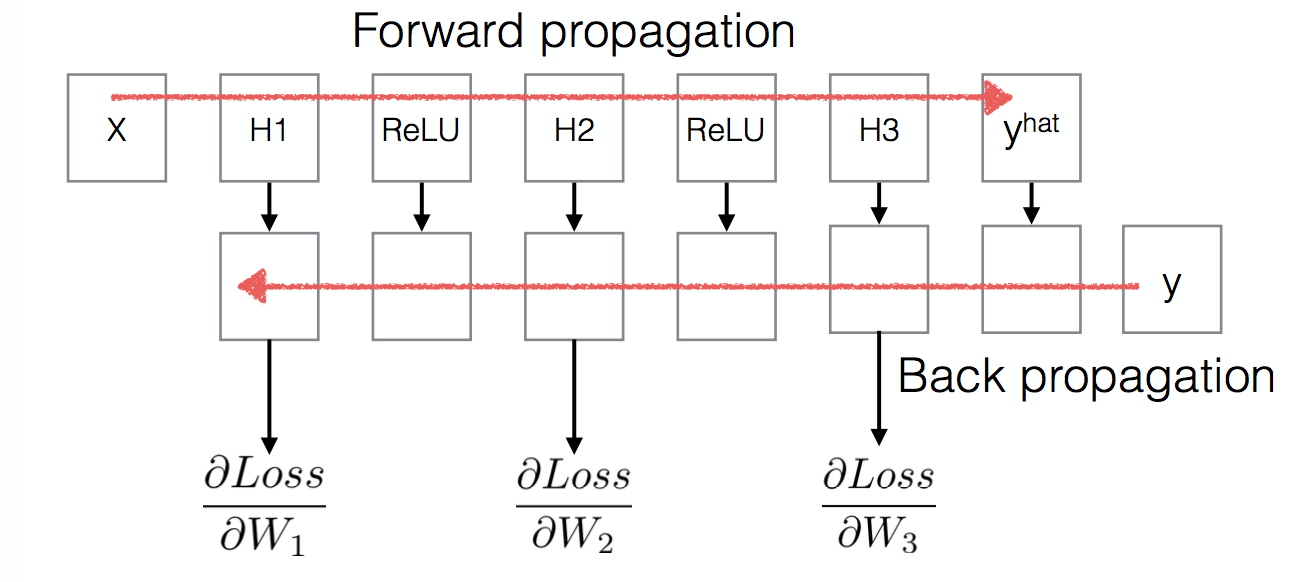
\includegraphics[width=.8\linewidth]{backpropagation.png}
%\end{center}
%\end{frame}
%
%
%\begin{frame}{Back-propagation}
%
%\alert{Forward pass:}
%
%\begin{center}
%	\begin{tikzpicture}
%	\tikzstyle{place}=[rectangle, draw=black, minimum size = 8mm]
%	\draw node at (0, 0) (input) {$X$};
%	\draw node at (2, 0) (h1) {$H_1$};
%	\draw node at (4, 0) (o1) {$O_1$};
%	\draw node at (6, 0) (h2) {$H_2$};
%	\draw node at (8, 0) (o2) {$O_2$};
%	\draw node at (10, 0) (output) {$\hat{y} $};
%	\draw node at (12, 0) (mse) {$MSE$};
%	
%	\draw [->]  (input) -- (h1) node[pos=.49, above] {$W_1$} ;
%	\draw [->]  (h1) -- (o1) node[pos=.49, above] {$f$} ;
%	\draw [->]  (o1) -- (h2) node[pos=.49, above] {$W_2$} ;
%	\draw [->]  (h2) -- (o2) node[pos=.49, above] {$f$} ;
%	\draw [->]  (o2) -- (output) node[pos=.49, above] {$W_3$} ;
%	\draw [->]  (output) to (mse);	
%	\end{tikzpicture}
%\end{center}
%	
%
%\vfill
%	
%\alert{Backward pass:}
%	
%\begin{center}
%	\begin{tikzpicture}
%		\draw node at (0, 0) (input) {$X$};
%		\draw node at (2, 0) (h1) {$H_1$};
%		\draw node at (4, 0) (o1) {$O_1$};
%		\draw node at (6, 0) (h2) {$H_2$};
%		\draw node at (8, 0) (o2) {$O_2$};
%		\draw node at (10, 0) (output) {$\hat{y} $};
%		\draw node at (12, 0) (mse) {$MSE$};
%		
%		\draw [->, dashed]   (h1)  -- (input) node[pos=.49, above] {$\frac{\partial H_1}{\partial X}$} ;
%		\draw [->, dashed]   (o1) -- (h1) node[pos=.49, above] {$\frac{\partial O_1}{\partial H_1}$} ;
%		\draw [->, dashed]   (h2) -- (o1) node[pos=.49, above] {$\frac{\partial H_2}{\partial O_1}$} ;
%		\draw [->, dashed]   (o2) -- (h2) node[pos=.49, above] {$\frac{\partial O_2}{\partial H_2}$} ;
%		\draw [->, dashed]   (output) -- (o2)node[pos=.49, above] {$\frac{\partial \hat{y}}{\partial O_2}$} ;
%		\draw [->, dashed]  (mse) -- (output) node[pos=.49, above] {$\frac{\partial MSE}{\partial \hat{y} }$} ;	
%		
%		\draw [->, dashed]  (9, -0.05) -- (9, -1.2)  node[pos=.49, right] {$\frac{\partial \hat{y}}{\partial W_3} = O_2^T$} ;
%		\draw [->, dashed]  (5, -0.05) -- (5, -1.2)  node[pos=.49, right] {$\frac{\partial H_2}{\partial W_2} = O_1^T$} ;
%		\draw [->, dashed]  (1, -0.05) -- (1, -1.2)  node[pos=.49, right] {$\frac{\partial H_1}{\partial W_1} = X^T$} ;
%	\end{tikzpicture}
%\end{center}
%\end{frame}
%
%
%
%\begin{frame}{Back-propagation}
%\alert{Forward pass:}
%
%\begin{center}
%	\begin{tikzpicture}
%	\tikzstyle{place}=[rectangle, draw=black, minimum size = 8mm]
%	\draw node at (0, 0) (input) {$X$};
%	\draw node at (2, 0) (h1) {$H_1$};
%	\draw node at (4, 0) (o1) {$O_1$};
%	\draw node at (6, 0) (h2) {$H_2$};
%	\draw node at (8, 0) (o2) {$O_2$};
%	\draw node at (10, 0) (output) {$\hat{y} $};
%	\draw node at (12, 0) (mse) {$MSE$};
%	
%	\draw [->]  (input) -- (h1) node[pos=.49, above] {$W_1$} ;
%	\draw [->]  (h1) -- (o1) node[pos=.49, above] {$\sigma$} ;
%	\draw [->]  (o1) -- (h2) node[pos=.49, above] {$W_2$} ;
%	\draw [->]  (h2) -- (o2) node[pos=.49, above] {$\sigma$} ;
%	\draw [->]  (o2) -- (output) node[pos=.49, above] {$W_3$} ;
%	\draw [->]  (output) to (mse);	
%	\end{tikzpicture}
%\end{center}
%
%\vfill
%
%\alert{Backward pass:}
%
%\begin{center}
%	\begin{tikzpicture}
%	\draw node at (0, 0) (input) {$X$};
%	\draw node at (2, 0) (h1) {$H_1$};
%	\draw node at (4, 0) (o1) {$O_1$};
%	\draw node at (6, 0) (h2) {$H_2$};
%	\draw node at (8, 0) (o2) {$O_2$};
%	\draw node at (10, 0) (output) {$\hat{y}$};
%	\draw node at (12, 0) (mse) {$MSE$};
%	
%	\draw [->, dashed]   (h1)  -- (input) node[pos=.49, above] {\scriptsize $W_1^T$} ;
%	\draw [->, dashed]   (o1) -- (h1) node[pos=.49, above] {\scriptsize $O_1 (1-O_1)$} ;
%	\draw [->, dashed]   (h2) -- (o1) node[pos=.49, above] {\scriptsize $W_2^T$} ;
%	\draw [->, dashed]   (o2) -- (h2) node[pos=.49, above] {\scriptsize $O_2 (1 - O_2)$} ;
%	\draw [->, dashed]   (output) -- (o2)node[pos=.49, above] {\scriptsize $W_3^T$} ;
%	\draw [->, dashed]  (mse) -- (output) node[pos=.49, above] {\scriptsize $-2(\hat{y} - y)$} ;	
%	
%	\draw [->, dashed]  (9, -0.05) -- (9, -1.2)  node[pos=.49, right] {$O_2^T$} ;
%	\draw [->, dashed]  (5, -0.05) -- (5, -1.2)  node[pos=.49, right] {$O_1^T$} ;
%	\draw [->, dashed]  (1, -0.05) -- (1, -1.2)  node[pos=.49, right] {$X^T$} ;
%	\end{tikzpicture}
%\end{center}
%\end{frame}
%
%
%
%\begin{frame}{Back-propagation}
%
%\begin{center}
%	\begin{tikzpicture}
%	\draw node at (0, 0) (input) {$X$};
%	\draw node at (2, 0) (h1) {$H_1$};
%	\draw node at (4, 0) (o1) {$O_1$};
%	
%	\only<3>{ 
%		\draw node at (0, 0) (input) {\color{red} $X$};
%		\draw node at (2, 0) (h1) {\color{red} $H_1$};
%		\draw node at (4, 0) (o1) {\color{red} $O_1$};
%	}
%	
%	\draw node at (6, 0) (h2) {$H_2$};
%	\draw node at (8, 0) (o2) {$O_2$};
%	
%	\only<2>{ 
%		\draw node at (6, 0) (h2) {\color{red}  $H_2$};
%		\draw node at (8, 0) (o2) {\color{red} $O_2$};	
%	}
%	
%	\draw node at (10, 0) (output) {$\hat{y}$};
%	\draw node at (12, 0) (mse) {$MSE$};
%	
%	\only<1>{ 
%		\draw node at (10, 0) (output) {\color{red} $\hat{y}$};
%		\draw node at (12, 0) (mse) {\color{red} $MSE$};	
%	}
%		
%	\draw [->, dashed]   (output) -- (o2)node[pos=.49, above] {\scriptsize $W_3^T$} ;
%	\draw [->, dashed]  (mse) -- (output) node[pos=.49, above] {\scriptsize $-2(\hat{y} - y)$} ;	
%	\draw [->, dashed]  (9, -0.05) -- (9, -1.2)  node[pos=.49, right] {$O_2^T$} ;
%		
%	\only<1>{ 
%		\draw [->, dashed, red]   (output) -- (o2)node[pos=.49, above] {\color{red} \scriptsize $W_3^T$} ;
%		\draw [->, dashed, red]  (mse) -- (output) node[pos=.49, above] {\color{red} \scriptsize $-2(\hat{y} - y)$} ;	
%		\draw [->, dashed, red]  (9, -0.05) -- (9, -1.2)  node[pos=.49, right] {\color{red} $O_2^T$} ;
%	}
%
%	\draw [->, dashed]   (h2) -- (o1) node[pos=.49, above] {\scriptsize $W_2^T$} ;
%	\draw [->, dashed]   (o2) -- (h2) node[pos=.49, above] {\scriptsize $O_2 (1 - O_2)$} ;
%	\draw [->, dashed]  (5, -0.05) -- (5, -1.2)  node[pos=.49, right] {$O_1^T$} ;
%	
%	\only<2>{ 
%		\draw [->, dashed, red]   (h2) -- (o1) node[pos=.49, above] {\color{red} \scriptsize $W_2^T$} ;
%		\draw [->, dashed, red]   (o2) -- (h2) node[pos=.49, above] {\color{red} \scriptsize $O_2 (1 - O_2)$} ;
%		\draw [->, dashed, red]  (5, -0.05) -- (5, -1.2)  node[pos=.49, right] {\color{red} $O_1^T$} ;
%	}
%
%	\draw [->, dashed]   (h1)  -- (input) node[pos=.49, above] {\scriptsize $W_1^T$} ;
%	\draw [->, dashed]   (o1) -- (h1) node[pos=.49, above] {\scriptsize $O_1 (1-O_1)$} ;
%	\draw [->, dashed]  (1, -0.05) -- (1, -1.2)  node[pos=.49, right] {$X^T$} ;
%
%	\only<3>{ 
%		\draw [->, dashed, red]   (h1)  -- (input) node[pos=.49, above] {\color{red} \scriptsize $W_1^T$} ;
%		\draw [->, dashed, red]   (o1) -- (h1) node[pos=.49, above] {\color{red} \scriptsize $O_1 (1-O_1)$} ;
%		\draw [->, dashed, red]  (1, -0.05) -- (1, -1.2)  node[pos=.49, right] {\color{red} $X^T$} ;
%	}	
%	\end{tikzpicture}
%\end{center}
%
%\vfill
%
%\begin{columns}
%	\begin{column}{.28\textwidth}
%		\alert{Шаг 1:}
%		\begin{equation*} 
%			\begin{aligned}
%				&  d = -2 (\hat{y} - y) \\
%				&  \frac{\partial MSE}{\partial W_3} = O_2^T \cdot d    \\
%			\end{aligned}
%		\end{equation*}
%	\end{column}
%	\begin{column}{.3\textwidth}
%		\only<2-4>{
%		\alert{Шаг 2:}
%		\begin{equation*} 
%			\begin{aligned}
%				&  d = d \cdot W_3^T * O_2 * (1 - O_2)  \\
%				&  \frac{\partial MSE}{\partial W_2} = O_1^T \cdot d \\
%			\end{aligned}
%		\end{equation*}}
%	\end{column}
%	\begin{column}{.35\textwidth}
%		\only<3-4>{
%		\alert{Шаг 3:}
%		\begin{equation*} 
%		\begin{aligned}
%		&  d = d \cdot W_2^T * O_1 * (1 - O_1)  \\
%		&  \frac{\partial MSE}{\partial W_1} = X^T \cdot d \\
%		\end{aligned}
%		\end{equation*}}
%	\end{column}
%\end{columns}
%
%\vfill
%
%\only<4>{  \alert{  Шаг SGD:}
%{\footnotesize
%\begin{columns}
%	\begin{column}{.28\textwidth}
%			\[  W_3^t = W_3^{t-1} - \eta \cdot \frac{\partial MSE}{\partial W_3}  \]
%	\end{column}
%	\begin{column}{.3\textwidth}
%			\[  W_2^t = W_2^{t-1} - \eta \cdot \frac{\partial MSE}{\partial W_2}  \]
%	\end{column}
%	\begin{column}{.35\textwidth}
%			\[  W_1^t = W_1^{t-1} - \eta \cdot \frac{\partial MSE}{\partial W_1}  \]
%	\end{column}
%\end{columns} 
%	}
%}
%\end{frame}
%
%
%
%\begin{frame}{Что такое слой в нейронной сети?}
%	\begin{wideitemize}
%		\item Любой слой - это какая-то абстракция, которая умеет делать прямой шаг и обратный шаг
%	
%		\item Для всех слоёв, которые мы дальше будем изучать, мы всегда будем смотреть на то как выглядят эти два шага
%	\end{wideitemize}
%\end{frame}
%
%
%\begin{frame}{А мне точно надо понимать backprop?}
%	\begin{wideitemize}
%		\item  \alert{Да, точно!} 
%				
%		\item  "Backprop – leaky abstraction!"
%		
%		\item  Почему сеть не обучается?
%		
%		\item  Почему сеть обучается слишком медленно? 
%		
%		\item  Какие проблемы могут возникать в обучении из-за плохой архитектуры? 
%	\end{wideitemize}
%\end{frame}

\end{document}

